 \documentclass{llncs}

%\documentclass[envcountsame, fleqn]{llncs}
\usepackage{amsmath, latexsym}
\usepackage{amsthm}
\usepackage{graphicx}
\usepackage{epic,eepic}

\pagestyle{plain}
\usepackage{listings}
\usepackage{psfrag}
\usepackage{rotating}

\usepackage{url}
\usepackage{amssymb,epsfig,amstext}
\usepackage{txfonts}
\usepackage{algorithmic}
\usepackage{algorithm}
\usepackage{graphicx}

\usepackage{todonotes}
\usepackage{multirow}
\usepackage{float,color}
\usepackage{picinpar,color,xcolor,wrapfig}
\setcounter{secnumdepth}{4}
\sloppy

\pagestyle{plain}

%%%%%%%%%%%%%%%   MACROS  %%%%%%%%%%%%%%%%%%


%!TEX root = popl2018.tex

\newcommand{\set}[1]{\{ #1 \}}
\newcommand{\sequence}[2]{(#1, \ldots, #2)}
\newcommand{\couple}[2]{(#1,#2)}
\newcommand{\pair}[2]{(#1,#2)}
\newcommand{\triple}[3]{(#1,#2,#3)}
\newcommand{\quadruple}[4]{(#1,#2,#3,#4)}
\newcommand{\tuple}[2]{(#1,\ldots,#2)}
\newcommand{\Nat}{\ensuremath{\mathbb{N}}}
\newcommand{\Rat}{\ensuremath{\mathbb{Q}}}
\newcommand{\Rea}{\ensuremath{\mathbb{R}}}
\newcommand{\Zed}{\ensuremath{\mathbb{Z}}}
%\newcommand{\true}{\top}
%\newcommand{\false}{\perp}
\newcommand{\bottom}{\perp}
%% \newcommand{\powerset}[1]{{\cal P}(#1)}
\newcommand{\npowerset}[2]{{\cal P}^{#1}(#2)}
\newcommand{\finitepowerset}[1]{{\cal P}_f(#1)}
\newcommand{\level}[2]{L_{#1}(#2)}
\newcommand{\card}[1]{\mbox{card}(#1)}
\newcommand{\range}[1]{\mathtt{ran}(#1)}
\newcommand{\astring}{s}

\newcommand{\Cc}{\mathcal{C}}


\newcommand {\notof}{\ensuremath{\neg}}
\newcommand {\myand}{\ensuremath{\wedge}}
\newcommand {\myor}{\ensuremath{\vee}}
\newcommand {\mynext}{\mbox{{\sf X}}}
\newcommand {\until}{\mbox{{\sf U}}}
\newcommand {\sometimes}{\mbox{{\sf F}}}
\newcommand {\previous}{\mynext^{-1}}
\newcommand {\since}{\mbox{{\sf S}}}
\newcommand {\fminusone}{\mbox{{\sf F}}^{-1}}
\newcommand {\everywhere}[1]{\mbox{{\sf Everywhere}}(#1)}



\newcommand{\aatomic}{{\rm A}}
\newcommand{\aset}{X}
\newcommand{\asetbis}{Y}
\newcommand{\asetter}{Z}

\newcommand{\avarprop}{p}
\newcommand{\avarpropbis}{q}
\newcommand{\avarpropter}{r}
\newcommand{\varprop}{{\rm PROP}} % Set of atomic propositions (for a given logic)

% formulae

\newcommand{\aformula}{\astateformula} % a formula
\newcommand{\aformulabis}{\astateformulabis} % another formula (when at least 2 are present)
\newcommand{\aformulater}{\astateformulater} % another formula (when at least 3 are present)
\newcommand{\asetformulae}{X}
\newcommand{\subf}[1]{sub(#1)}

\newcommand{\aautomaton}{{\mathbb A}}
\newcommand{\aautomatonbis}{{\mathbb B}}

\newcommand {\length}[1] {\ensuremath{|#1|}}



% Equivalences
\newcommand{\egdef}{\stackrel{\mbox{\begin{tiny}def\end{tiny}}}{=}} % =def=
\newcommand{\eqdef}{\stackrel{\mbox{\begin{tiny}def\end{tiny}}}{=}} % =def=
\newcommand{\equivdef}{\stackrel{\mbox{\begin{tiny}def\end{tiny}}}{\equivaut}} % <=def=>
\newcommand{\equivaut}{\;\Leftrightarrow\;}

\newcommand{\ainfword}{\sigma}

\newcommand{\amap}{\mathfrak{f}}
\newcommand{\amapbis}{\mathfrak{g}}

\newcommand{\step}[1]{\xrightarrow{\!\!#1\!\!}}
\newcommand{\backstep}[1]{\xleftarrow{\!\!#1\!\!}}

\newcommand {\aedge}[1] {\ensuremath{\stackrel{#1}{\longrightarrow}}}
\newcommand {\aedgeprime}[1] {\ensuremath{\stackrel{#1}{\longrightarrow'}}}
\newcommand {\afrac}[1] {\ensuremath{\mathit{frac}(#1)}}
\newcommand {\cl}[1] {\ensuremath{\mathit{cl}(#1)}}
\newcommand {\sfc}[1] {\ensuremath{\mathit{sfc}(#1)}}
\newcommand {\dunion} {\ensuremath{\uplus}}
\newcommand {\edge} {\ensuremath{\longrightarrow}}
\newcommand {\emptyword}{\ensuremath{\epsilon}}
\newcommand {\floor}[1] {\ensuremath{\lfloor #1 \rfloor}}
\newcommand {\intersection} {\ensuremath{\cap}}
\newcommand {\union} {\ensuremath{\cup}}
\newcommand {\vals}[2] {\ensuremath{\mathit{val}_{#2}(#1)}}



\newcommand {\pspace} {\textsc{pspace}}
\newcommand {\nlogspace} {\textsc{nlogspace}}
\newcommand {\logspace} {\textsc{logspace}}
\newcommand {\expspace} {\textsc{expspace}}
\newcommand {\np} {\textsc{np}}
\newcommand {\threeexptime} {\textsc{3exptime}}
\newcommand {\polytime} {\textsc{p}}
\newcommand{\twoexpspace}{\textsc{2expspace}}
\newcommand{\threeexpspace}{\textsc{3expspace}}
\newcommand {\nexptime} {\textsc{nexptime}}



\newcommand{\aalphabet}{\Sigma}     % an alphabet, A is already used for atoms
\newcommand{\aword}{\mathfrak{u}}
\newcommand{\awordbis}{\mathfrak{v}}



\newcommand{\aassertion}{P}
\newcommand{\aassertionbis}{Q}
\newcommand{\aexpression}{e}
\newcommand{\aexpressionbis}{f}
\newcommand{\avariable}{\mathtt{x}}
\newcommand{\uniquevar}{\mathtt{u}}
\newcommand{\uniquevarbis}{\mathtt{v}}
\newcommand{\avariablebis}{\mathtt{y}}
\newcommand{\avariableter}{\mathtt{z}}
\newcommand{\nullconstant}{\mathtt{null}}
\newcommand{\nilvalue}{nil}
\newcommand{\emptyconstant}{\mathtt{emp}}
\newcommand{\infheap}{\mathtt{inf}}
\newcommand{\saturated}{\mathtt{Saturated}}

\newcommand{\astateformula}{\phi}
\newcommand{\astateformulabis}{\psi}
\newcommand{\astateformulater}{\varphi}
%%
\newcommand{\separate}{\ast}
\newcommand{\sep}{\separate}
\newcommand{\size}{\mathtt{size}}
\newcommand{\sizeeq}[1]{\mathtt{size} \ = \ #1}
\newcommand{\alloc}[1]{\mathtt{alloc}(#1)}
\newcommand{\allocb}[2]{\mathtt{alloc}^{-1}[#2](#1)}
\newcommand{\isol}[1]{\mathtt{isoloc}(#1)}
\newcommand{\icell}{\mathtt{isocell}}
\newcommand{\malloc}{\mathtt{malloc}}
\newcommand{\cons}{\mathtt{cons}}
\newcommand{\new}{\mathtt{new}}
\newcommand{\free}[1]{\mathtt{free} \ #1}
\newcommand{\maxform}[1]{\mathtt{maxForms}(#1)}
\newcommand{\locations}[1]{\mathtt{loc}(#1)}
\newcommand{\values}{\mathtt{Val}}
\newcommand{\aheap}{\mathfrak{h}}
\newcommand{\avaluation}{\mathfrak{V}}
\newcommand{\heaps}{\mathcal{H}}
\newcommand{\astore}{\mathfrak{s}}
\newcommand{\stores}{\mathcal{S}}
\newcommand{\amodel}{\mathfrak{M}}
\newcommand{\alabel}{\ell}

\newcommand{\aprogram}{\mathtt{PROG}}
\newcommand{\programs}{\mathtt{P}}
\newcommand{\ctprograms}{\programs^{ct}}
\newcommand{\aninstruction}{\mathtt{instr}}
\newcommand{\ainstruction}{\mathtt{instr}}
\newcommand{\instructions}{\mathtt{I}}
\newcommand{\aguard}{\ensuremath{g}}
\newcommand{\guards}{\ensuremath{G}}
\newcommand{\domain}[1]{\mathtt{dom}(#1)}
\newcommand{\memory}{\stores\times\heaps}
\newcommand{\skipinstruction}{\mathtt{skip}}

\newcommand{\execution}{\mathtt{comp}}
\newcommand{\aux}{\mathtt{embd}}
\newcommand{\runof}{run}
\newcommand{\anexecution}{e}


\newcommand{\aletter}{\ensuremath{a}}
\newcommand{\aletterbis}{\ensuremath{b}}
\newcommand{\alocation}{\mathfrak{l}}

\newcommand{\pointsl}[1]{\stackrel{#1}{\hookrightarrow}}
\newcommand{\ppointsl}[1]{\stackrel{#1}{\mapsto}}
\newcommand{\ourhook}[1]{\stackrel{#1}{\hookrightarrow}}
\newcommand{\ltrue}{{\sf true}}
\newcommand{\lfalse}{{\sf false}}


\newcommand{\variables}{\mathtt{FVAR}}
\newcommand{\pvariables}{\mathtt{PVAR}}
\newcommand{\secvariables}{\mathtt{SVAR}}
\newcommand{\logique}[1]{\mathtt{FO}(#1)}



\newcommand{\atranslation}{\mathfrak{t}}
\newcommand{\nbpred}[1]{\widetilde{\sharp #1}}
\newcommand{\nbpredstar}[1]{\widetilde{\sharp #1}^{\star}}
\newcommand{\isolated}{\mathtt{isol}}
\newcommand{\stdmarks}{\mathtt{envir}}
\newcommand{\relation}[1]{\mathtt{relation}_{#1}}
\newcommand{\freevar}{\mathtt{FV}}
\newcommand{\notonmark}{\mathtt{notonenv}}
\newcommand{\InVal}[1]{\mathtt{InVal}\!\left(#1\right)}
\newcommand{\NotOnEnv}[1]{\mathtt{NotOnEnv}\!\left(#1\right)}
\newcommand{\PartOfVal}[1]{\mathtt{PartOfVal}\!\left(#1\right)}
%\newcommand{\nbpreds}[3]{\sharp #1 \geq #2}
\newcommand{\defstyle}[1]{{\emph{#1}}}

\newcommand{\cut}[1]{}
\newcommand{\interval}[2]{[#1,#2]}
\newcommand{\buniquevar}{\overline{\uniquevar}}
\newcommand{\bbuniquevar}{\overline{\overline{\uniquevar}}}
\newcommand{\magicwand}{\mathop{\mbox{$\mbox{$-~$}\!\!\!\!\ast$}}}
\newcommand{\wand}{\magicwand}
\newcommand{\septraction}{\stackrel{\hsize0pt \vbox to0pt{\vss\hbox to0pt{\hss\raisebox{-6pt}{\footnotesize$\lnot$}\hss}\vss}}{\magicwand}}
%% \newcommand{\reach}{\mathtt{reach}}
\mathchardef\mhyphen="2D % hyphen while in math mode

\newcommand{\adataword}{\mathfrak{dw}}
\newcommand{\adatum}{\mathfrak{d}}

\newcommand{\collectionknives}{\mathtt{ks}}
\newcommand{\collectionknivesfork}[1]{\mathtt{ksfs}_{=#1}}
\newcommand{\collectionknivesforks}{\mathtt{ksfs}}
\newcommand{\collectionkniveslargeforks}{\mathtt{kslfs}}


\newcommand{\acounter}{\mathtt{C}}

\newcommand{\fotwo}[3]{{\mbox{FO2}_{#1,#2}(#3)}}
\newcommand{\mtrans}[1]{t\!\left(#1\right)^{\Box}}
\newcommand{\mbtrans}[2]{\mtrans{#2}_{#1}}


\newcommand{\alogic}{\mathfrak{L}}


\newcommand{\semantics}[1]{\ensuremath{[ #1 ]}}


\newcommand{\adomino}{\mathfrak{d}}
\newcommand{\atile}{\mathfrak{d}}
\newcommand{\atiling}{\mathfrak{t}}

\newcommand{\hori}{\mathtt{h}}
\newcommand{\verti}{\mathtt{v}}
\newcommand{\domi}{\mathtt{d}}

\newcommand{\cpyrel}{\mathfrak{cp}}

\newcommand{\cntcmp}{\mathfrak{C}}

\newcommand{\heapdag}{\mathfrak{G}}

\newcommand{\onmainpath}{\mathtt{mp}}

\newcommand{\tree}{\mathtt{tree}}

%\newcommand{\tile}{\mathtt{tile}}

\newcommand{\type}{\mathtt{type}}

\newcommand{\ptype}{\mathtt{ptype}}

\newcommand{\exttype}{\mathtt{exttype}}

\newcommand{\anctypes}{\mathtt{AncTypes}}

\newcommand{\destypes}{\mathtt{DesTypes}}

\newcommand{\inctypes}{\mathtt{IncTypes}}

\newcommand{\treeic}{\mathtt{treeIC}}

\newcommand{\trs}{\mathfrak{trs}}


\newcommand{\nin}{\not \in}
\newcommand{\cupplus}{\uplus}
\newcommand{\aunarypred}{\mathtt{P}}


\newcommand{\hide}[1]{}

\newcommand{\eval}[2]{\llbracket#1\rrbracket_{#2}}
\newcommand\cur{\mathsf{cur}}
\newcommand\dom{\mathsf{dom}}
\newcommand\rng{\mathsf{rng}}

\newcommand\dd{\mathbb{D}}
\newcommand\nat{\mathbb{N}}


\newcommand\cA{\mathcal{A}}
\newcommand\cB{\mathcal{B}}
\newcommand\cC{\mathcal{C}}
\newcommand\cE{\mathcal{E}}
\newcommand\cG{\mathcal{G}}
\newcommand\Ll{\mathcal{L}}
\newcommand\cM{\mathcal{M}}
\newcommand\cP{\mathcal{P}}
\newcommand\cR{\mathcal{R}}
\newcommand\cS{\mathcal{S}}
\newcommand\cT{\mathcal{T}}

\newcommand\vard{\mathfrak{d}}

\newcommand\replaceall{\mathsf{replaceAll}}
\newcommand\indexof{\mathsf{IndexOf}}


\newcommand\strline{\mathsf{SL}}

\newcommand\pstrline{\mathsf{SL_{pure}}}

\newcommand\search{\mathsf{search}}

\newcommand\verify{\mathsf{verify}}

\newcommand\searchleft{\mathsf{searchLeft}}

\newcommand\searchlong{\mathsf{searchLong}}


\newcommand\pref{\mathsf{Pref}}

\newcommand\wprof{\mathsf{WP}}

\newcommand\vars{\mathsf{Vars}}

\newcommand\dep{\mathsf{Dep}}
\newcommand\ptn{\mathsf{Ptn}}

\newcommand\src{\mathsf{src}}
\newcommand\strtorep{\mathsf{strToRep}}

\newcommand\rpleft{\mathsf{l}}
\newcommand\rpright{\mathsf{r}}


\newcommand\srcnd{\mathsf{srcND}}

\newcommand\ctxt{\mathsf{ctxt}}


\newcommand\ctxts{\mathsf{Ctxts}}

\newcommand\sprt{\mathsf{sprt}}

\newcommand\val{\mathsf{val}}

\newcommand\srclen{\mathsf{srcLen}}

\newcommand\rpleftlen{\mathsf{lLen}}


\newcommand\dfs{\mathsf{DFS}}

\newcommand\repr{\mathsf{rep}}

\newcommand\red{\mathsf{red}}

\newcommand\gfun{\mathcal{F}}


\newcommand{\leftmost}{{\sf leftmost}}
\newcommand{\longest}{{\sf longest}}

\newcommand{\arbidx}{{\sf Idx_{arb}}}
\newcommand{\dmdidx}{{\sf Idx_{dmd}}}
\newcommand{\lftlen}{{\sf Len_{lft}}}

%\newtheorem{remark}[theorem]{Remark}


%%%%%%%%%%%%%%%%%%%%%%%%%%%%%%%%%%%%%%%%%%%%



\title{Decision procedure for string constraints \\
involving the integer data type}


\author{}

\institute{ }

\begin{document}


\maketitle

\begin{abstract}
In this note, we consider straight-line string constraints involving string and integer data types. 
%We define both the concrete and abstract version of the straight-line fragment. 
We propose semantic conditions and a generic decision procedure for the path feasibility of the symbolic execution of programs satisfying the semantic conditions. 
Furthermore, we show that common string operations,  including concat, replaceall, transducers, reverse, substring, indexof, and length, satisfy the semantic conditions.
%the concrete version of straight-line fragment satisfies the semantic conditions, thus enjoys a decidable satisfiability problem. 
Our approach is based on a variant of cost register automata.
\end{abstract}

\section{Introduction}
%\label{intro}
%
%\section{Preliminaries}
%\label{prel}
%
%Definition for NFA, NFT.

\section{Preliminaries}

For $n \in \nat$ with $n \ge 1$, we use $[n]$ to denote $\{1, \cdots, n\}$.

A string over $\Sigma$ is a (possibly empty) sequence of elements from $\Sigma$. Let $w=a_1\cdots a_n$ be a string. The reserve of $w$, denoted by $w^{(r)}$, is $a_n \cdots a_1$.

We consider two data types, the string data type and the integer data type. We will use $c, d,\dots$ to denote integer constants, $u, v, \dots$ to denote string constants,  $i, j, \dots$ to denote the  integer variables, and $x, y, \dots$ to denote the string variables.

A finite automaton (FA) $\Aut$ is a tuple $(Q, \Sigma, \delta, I, F)$, where $Q$ is a finite set of states, $\Sigma$ is a finite alphabet, $\delta \subseteq Q \times \Sigma \times Q$ is the transition relation, $I,F \subseteq Q$ are the set of initial and final states respectively. A string $w=\sigma_1 \cdots \sigma_n$ is accepted by $\Aut$ if there is a state sequence $q_0 \cdots q_n$ such that $q_0 \in I$, $q_n \in F$, and $(q_{i-1}, \sigma_i, q_i) \in \delta$ for each $i \in [n]$. In particular, an empty string $\varepsilon$ is accepted by $\Aut$ if $I \cap F \neq \emptyset$. The language defined by $\Aut$, denoted by $\Lang(\Aut)$, is defined as the set of strings accepted by $\Aut$.

A finite transducer (FT) $T$ is a tuple $(Q, \Sigma, \delta, I, F)$, where $Q$ is a finite set of states, $\Sigma$ is a finite alphabet, $\delta$ is the transition relation, which is a finite subset of $Q \times \Sigma \times Q \times \Sigma^*$, $I,F \subseteq Q$ are the set of initial and final states respectively. For readability, we write a transition $(q, \sigma, q', u)$ as $q \xrightarrow{\sigma, u} q'$. A run of $T$ over a string $w=\sigma_1 \cdots \sigma_n$ is a state sequence of transitions $q_0 \xrightarrow{\sigma_1, u_1} q_1 \cdots q_n \xrightarrow{\sigma_n, u_n} q_n$. The run is accepting if $q_0 \in I$ and $q_n \in F$. The string $u_1 \cdots u_n$ is called the output of the run. We use $\cT(T)$ to denote the set of pairs $(w, u)$ such that there is an accepting run of $T$ on $w$, with the output $u$.

A linear arithmetic formula $\phi$ is defined by the rules: $\phi::= t \ o \ t \mid \neg \phi \mid \phi \vee \phi \mid \exists i.\ \phi$, where $o \in \{=, \neq, \le, \ge, <, >\}$ and $t$ is defined by the rules $t::= i \mid c \mid ct \mid t + t $.  
For a quantifier free linear integer arithmetic formula $\phi$ that contains the free variables $i_1, \cdots, i_k$, we use $\cM(\phi)$ to denote the set of models of $\phi$, namely, $\{(c_1, \cdots ,c_k) \mid \phi[c_1/i_1, \cdots, c_k/i_k] \mbox{ holds}\}$. An existential linear arithmetic formula is a linear arithmetic formula where all the existential quantifiers are under the scope of even number of negation symbols.

\section{The logic \slint}


We consider two types of functions, string functions that return strings and integer functions that return integers. Specifically, we consider 
\begin{itemize}
\item string functions $f(x_1, \vec{i_1}, \cdots, x_k, \vec{i_k})$, where $f$ is of the arity $\Sigma^* \times \intnum^{n_1} \times \cdots \times \Sigma^* \times \intnum^{n_k} \rightarrow 2^{\Sigma^*}$, and
\item  integer functions $g(x_1, \vec{i_1}, \cdots, x_k, \vec{i_k})$, where $g$ is of the arity $\Sigma^* \times \intnum^{n_1} \times \cdots \times \Sigma^* \times \intnum^{n_k} \rightarrow 2^\intnum$.
\end{itemize} 
Note that $f$ and $g$ can be nondeterministic.
%\subsection{The abstract version}

We consider string constraints where the formulae are of the form $S \wedge A$ defined by the following rules,
\[
\begin{array}{l c l}
t  &::=& i \mid c \mid  g(x_1, \vec{t_1}, \cdots, x_k, \vec{t_k}) \mid ct \mid t + t,   \\
S &::= &  x:=f(x_1, \vec{t_1}, \cdots, x_k, \vec{t_k}) \mid S;S, \\
A_r & ::= & x \in \Aut  \mid A_r \wedge A_r, \\
A_i & ::= & t\ o\ t \mid A_i \wedge A_i \mid A_i \vee A_i,\\
A & ::= &   A_r \wedge A_i, 
\end{array}
\]
where $f$ is a string function and $g$ is an integer function, $\vec{t_j} = t_{j,1}, \cdots, t_{j, n_j}$ for each $j \in [k]$, $\Aut$ is a finite-state automaton, and $o \in \{=, \neq, \ge, \le, >, <\}$.

The logic {\slint} is defined as straight-line fragment of the aforementioned string constraints, specifically, {\slint} is defined as the collection of the formulae $S \wedge A$ satisfying that {\bf $S$ is in single static assignment (SSA) form}.  Note that in {\slint}, the straight-line restriction is applied only on $S$, which contains only the assignments to string variables (but not integer variables). No restrictions are put on the integer constraints in $A_i$.
%Intuitively speaking, the integer constraints in $S \wedge A$ are split into the integer assignments in $S$ where the right-hand side is of the form $g(x_1, \vec{i_1}, \cdots, x_k, \vec{i_k})$ and the constraints $t\ o\ t$ in $A$ where the integer functions $g$ do not occur.
%\begin{itemize}
%\item $S$ is in single static assignment (SSA) form,
%\item all the assignments $i: = t$ in $S$ satisfy that either $t$ is of the form $g(x_1, \vec{i_1}, \cdots, x_k, \vec{i_k})$, or $t$ contains no occurrences of the functions of the form $g(x_1, \vec{i_1}, \cdots, x_k, \vec{i_k})$, namely, $t$ is an integer term built from integer variables and constants ,
%
%\item $A$ contains no occurrences of the functions $g(x_1, \vec{i_1}, \cdots, x_k, \vec{i_k})$,
%
%\item all the string variables in $A$ also occur in $S$.
%\end{itemize} 

%%%%%%%%%%%%%%%%%%%%%%%%%%%%%%%%%%%%%%%%%%%%%%%%%%
%%%%%%%%%%%%%%%%%%%%%%%%%%%%%%%%%%%%%%%%%%%%%%%%%%
\hide{
\subsection{The concrete version}

SL$_{int}$ comprises all the formulae $S \wedge A$ defined by the following rules,
\[
\begin{array}{l c l}
t  &::=& i \mid c \mid \length(x) \mid \indexof_u(x, i) \mid t + t,   \\
S &::= & i:= t \mid x := \substring(y, i, j)  \mid x:= y \concat z \mid x:= \replaceall_{e,u}(y) \mid\\
&&  x:=\reverse(y) \mid x:=T(y) \mid S;S, \\
A & ::= &   x \in \Aut \mid t\ o\ t \mid A \wedge A,
\end{array}
\]
where $c$ is an integer constant, $e$ is a regular expression,  $u$ is a string constant, $T$ is an NFT, $\Aut$ is an NFA, and $o \in \{=, \neq, \le, \ge, <, >\}$.
Note that $\replaceall_{e,u}$ is the replaceAll function where $e$ and $u$ are the pattern and the replacement parameters.

For technical convenience, we assume that 
\begin{itemize}
\item $S$ is in single static assignment (SSA) form,
%
\item all the assignments $i: = t$ in $S$ satisfy that either $t = \length(x)$, $t=\indexof_u(x, j)$, or $t$ contains no occurrences of these two functions,
%
\item $A$ contains no occurrences of the functions $\length$ or $\indexof$,
%
\item all the variables in $A$ also occur in $S$.
\end{itemize} 
}
%%%%%%%%%%%%%%%%%%%%%%%%%%%%%%%%%%%%%%%%%%%%%%%%%%
%%%%%%%%%%%%%%%%%%%%%%%%%%%%%%%%%%%%%%%%%%%%%%%%%%

\begin{example}
The formula $x:= y \concat z \wedge y := \substring(y', \indexof(x, c), j)  \wedge y' \in (ab)^* \wedge z \in a^* c b^* \wedge   j = 2 \indexof(x, c)$ belongs to \slint.
\end{example}

In the next section, we specify the semantic conditions for {\slint} in order to achieve decision procedures. For this purpose, we need the concepts of cost-enriched regular languages and recognisable relations. 

\section{The semantic conditions}

\subsection{Cost-enriched regular languages and recognisable relations}

A cost-enriched string is $(w, (n_1, \cdots, n_k))$ with a string $w$ and $n_i \in \intnum$ for all $i \in [k]$. 
A cost-enriched language $L$ is a subset of $\Sigma^* \times \intnum^k$ for some $k$. Note that all the cost-enriched strings in $L$ have the same number of costs, namely $k$.
A cost-enriched relation $\cR$ is a subset of $\Sigma^* \times \intnum^{k_1} \times \cdots \Sigma^* \times \intnum^{k_l}$.

\begin{definition}[Cost-enriched finite automata and regular languages]
A cost-enriched finite automaton (CEFA) $\Aut$ is a tuple $(Q, \Sigma, R, \delta, I, F)$ where $Q, \Sigma, I, F$ are as in FA, $R=(r_1, \cdots, r_k)$ is a vector of (mutually distinct) registers, $\delta$ is the transition relation which is a finite set of tuples $(q, \sigma, q', \eta)$ where $q, q' \in Q$, $\sigma \in \Sigma$, and $\eta: R \rightarrow \intnum$ is the cost-update function. For convenience, we usually write $(q, \sigma, q', \eta) \in \Delta$ as $q \xrightarrow{\sigma, \eta} q'$.
\\
A cost-enriched string $(w, (n_1, \cdots,n_k)) \in \Sigma^* \times \intnum^k$ with $w=\sigma_1 \cdots \sigma_m$ is accepted by $\Aut$ if there is a sequence of transitions $q_0 \xrightarrow{\sigma_1, \eta_1} q_1 \cdots q_{m-1} \xrightarrow{\sigma_m, \eta_m} q_m$ such that $n_i = \eta_1(r_i) + \cdots + \eta_m(r_i)$ for each $i \in [k]$. The set of cost-enriched strings accepted by $\Aut$ is denoted as $\Lang(\Aut)$. A cost-enriched language $L \subseteq \Sigma^* \times \intnum^k$ is called a cost-enriched regular language (CERL) if there is a CEFA $\Aut$ such that $L = \Lang(\Aut)$.
\end{definition}
CEFA can be seen as a variant of CRA in \cite{RLJ+13}, by allowing nondeterminism and disallowing  partial final cost functions. 

For a CEFA $\Aut$, we use $R(\Aut)$ to denote the vector of registers occurring in $\Aut$. Moreover, for a CEFA $\Aut$ and a vector of integer variables $\vec{i}$ such that $R(\Aut) \cap \vec{i} = \emptyset$, we use $\Aut[\vec{i}/R(\Aut)]$ to denote the CEFA obtained from $\Aut$ by replacing the registers in $R(\Aut)$ with those from $\vec{i}$. 

%Let $\Aut = (Q, \Sigma, R, \delta, I, F)$ be a CEFA and $I',F' \in Q$. Then we use $\Aut_{I', F'}$ to denote the CEFA $(Q, \Sigma, R, \delta, I', F')$.

Given two CEFAs $\Aut_1 = ( Q_1, \Sigma, R_1, \delta_1, I_1, F_1)$ and $\Aut_2 = (Q_2, \Sigma, \delta_2, R_2, I_2, F_2)$ with $R_1 \cap R_2 = \emptyset$, we define the product of $\Aut_1$ and $\Aut_2$, denoted by $\Aut_1 \times \Aut_2$, as $(Q_1 \times Q_2, \Sigma, R_1 \cup R_2, \delta, I_1 \times I_2, F_1 \times F_2)$ such that $\delta$ comprises the tuples $((q_1, q_2), \sigma, (q'_1, q'_2), \eta)$ satisfying that $(q_1, \sigma, q'_1, \eta_1) \in \delta_1$, $(q_2, \sigma, q'_2, \eta_2) \in \delta_2$, and $\eta = \eta_1\cup \eta_2$ for some $\eta_1, \eta_2$.

%Note that according to the definition, over each word $w$, $\Aut^{(r)}(w) = \Aut(w)$. 

\begin{definition}[LA-SAT w.r.t. CEFA]\label{def-la-sat-cefa}
Let $\Aut_1=(Q_1, \Sigma, R_1, \delta_1, I_1, F_1)$, $\cdots$, $\Aut_k=(Q_k, \Sigma, R_k, \delta_k, I_k, F_k)$ be CEFAs
%  with $R_i = (r_{i,1}, \cdots, r_{i, l_i})$ for each $i \in [k]$, 
  and $\phi$ be a quantifier-free linear arithmetic formula whose free variables are from  $R_1 \cup \cdots \cup R_k \cup X$ for some $X$ such that $X \cap (R_1 \cup \cdots \cup R_k) = \emptyset$. Then $\phi$ is said to be satisfiable w.r.t. $\Aut_1, \cdots, \Aut_k$ if  there are words $w_1, \cdots, w_k$ and an assignment function $\eta: R_1 \cup \cdots R_k \cup X \rightarrow \intnum$  %integers $\vec{c_1} \in \intnum^{|R_1|}, \cdots, \vec{c_k} \in \intnum^{|R_k|}$, $\vec{d} \in \intnum^{|X|}$
 such that  $(w_1, \eta(R_1)) \in \Lang(\Aut_1)$, $ \cdots$, $(w_k, \eta(R_k)) \in \Lang(\Aut_k)$, and $\phi[\eta(R_1)/R_1, \cdots,\eta(R_k)/R_k, \eta(X)/X]$ holds.
\end{definition}
Note that in Definition~\ref{def-la-sat-cefa}, it may happen that $R_i \cap R_j \neq \emptyset$ for some $i, j \in [k]$ with $i \neq j$.

\begin{theorem}\label{thm-incra-la-sat}
The LA-SAT w.r.t. CEFA problem is decidable.
\end{theorem}

For the proof of Theorem~\ref{thm-incra-la-sat}, we state and prove the following lemma. 

\begin{lemma}\label{lem-incra-la}
Let $\Aut=(Q, \Sigma, R, \delta, I, F)$ be a CEFA with $R= (r_1, \cdots,  r_m)$. Then there is an existential linear arithmetic formula $\varphi_\Aut(r_1, \cdots, r_m)$ such that $\cM(\varphi_\Aut)= \{(c_1, \cdots, c_m) \mid \mbox{there exists } w \mbox{ such that } (w, c_1, \cdots, c_m) \in \Lang(\Aut)\}$.
\end{lemma}

\begin{proof}
Let $\delta = \{\tau_1, \cdots, \tau_l\}$ such that $\tau_j = (p_j, \sigma_j, p'_j, \eta_j)$ and $\eta_j(r_i) =  c_{i,j}$ for each $j \in [l]$ and $i \in [m]$.
According the results on FA, we know that for each pair of states $(q, q') \in I \times F$,  an existential linear arithmetic formula $\varphi_{q,q'}(j_1, \cdots, j_l)$ can be computed in linear time such that $\cM(\varphi_{q,q'})$ is the set of Parikh images of the transition sequences of $\Aut$ starting from $q$ and ending at $q'$. 

Then 
\[\varphi_\Aut(r_1, \cdots, r_m) ::= \bigvee \limits_{(q,q') \in I \times F} \exists j_1 \cdots \exists j_l.\ \left(\varphi_{q,q'}(j_1, \cdots, j_l) \wedge \bigwedge \limits_{i \in [m]} r_i = \sum \limits_{j \in [l]} c_{i,j} j_j \right).\]
\qed
\end{proof}

\begin{proof}[Theorem~\ref{thm-incra-la-sat}]
Let $\Aut_1=(Q_1, \Sigma, R_1, \delta_1, I_1, F_1)$, $\cdots$, $\Aut_k=(Q_k, \Sigma, R_k, \delta_k, I_k, F_k)$ be CEFAs and $\phi$ be a quantifier-free linear arithmetic formula whose free variables are from  $R_1 \cup \cdots \cup R_k \cup X$ for some $X$ such that $X \cap (R_1 \cdots R_k) = \emptyset$.
Suppose that for each $i \in [k]$, $R_i = (r_{i, 1}, \cdots, r_{i, l_i})$. Then the satisfiability of $\phi$ w.r.t. $\Aut_1,\cdots, \Aut_k$ can be reduced to the satisfiability problem of the  existential linear arithmetic formula
$
\phi \wedge \bigwedge \limits_{i \in [k]} \varphi_{\Aut_i}(r_{i,1}, \cdots, r_{i, l_i}).
$
\qed
\end{proof}

\begin{definition}[Cost-enriched recognisable relations]
A cost-enriched relation $\cR \subseteq \Sigma^* \times \intnum^{k_1} \times \cdots  \times \Sigma^* \times \intnum^{k_l}$ is a cost-enriched recognisable relation (CERR)  if it is a finite union of products of cost-enriched regular languages, namely, 
\[\cR = \bigcup \limits_{i=1}^n L_{i,1 } \times \cdots \times L_{i, l},\]
where $L_{i,1} \subseteq \Sigma^* \times \intnum^{k_1}, \cdots, L_{i, l} \subseteq \Sigma^* \times \intnum^{k_l}$ are CERL. 
A CEFA representation of $\cR$ is a collection of CERA tuples $(\Aut_{i,1}, \cdots, \Aut_{i,l})_{i \in [n]}$ such that $\Lang(\Aut_{i,j}) = L_{i,j}$ for each $i \in [n]$ and $j \in [l]$.
\end{definition}



\subsection{The two semantic conditions}
%The first semantic condition we put is as follows: The relation defined by the integer functions $g(x_1, \vec{i_1}, \cdots, x_k, \vec{i_k})$ is 

For specifying the semantic conditions, we introduce two additional concepts. 

\begin{definition}[CERR linear integer functions]
An integer function $g: \Sigma^* \times \intnum^{k_1} \times \Sigma^* \times \intnum^{k_l} \rightarrow 2^\intnum$ is a CERR linear integer function if there is a pair $(\cR, t)$ such that $\cR \subseteq \Sigma^* \times \intnum^{k_1+1} \times \Sigma^* \times \intnum^{k_l+1}$ is a CERR and $t$ a linear integer term over $r^{(1)}, \cdots, r^{(l)}$ such that for all $\vec{c_1} \in \intnum^{k_1}, \cdots, \vec{c_l} \in \intnum^{k_l}$, and $d_1 \in \intnum, \cdots, d_l \in \intnum$, it holds that $(w_1, (\vec{c_1}, d_1), \cdots, w_l, (\vec{c_l}, d_l)) \in \cR$ iff $t[d_1/r^{(1)}, \cdots, d_l/r^{(l)}] \in g(w_1, \vec{c_1}, \cdots, w_l, \vec{c_l})$.  For a CERR linear integer function $g$ witnessed by the pair $(\cR, t)$, a CEFA representation of $g$ is a tuple $((\Aut_{i,1}, \cdots, \Aut_{i, l})_{i \in [n]}, t)$, where $(\Aut_{i,1}, \cdots, \Aut_{i, l})_{i \in [n]}$ is a CEFA representation of $\cR$.

\end{definition}

\begin{example}
The string functions $\length$ and $\indexof_u$ are CERR linear integer functions, whose CEFA representations can be found in Section~\ref{sec-cslint}.
\end{example}

\begin{definition}[Cost enriched pre-image of CERL]
Suppose that $f: \Sigma^* \times \intnum^{k_1} \times \cdots \times \Sigma^* \times \intnum^{k_l} \rightarrow 2^{\Sigma^*}$ is a string function, $L \subseteq \Sigma^* \times \intnum^n$ is a CERL, and $L = \Lang(\Aut)$ for some CEFA $\Aut=(Q, R, \delta, I, F)$ where $R= (r_1, \cdots, r_n)$. Then the $R$-cost enriched pre-image of $L$ under $f$ is a pair $(\cR, \vec{t})$ such that 
\begin{itemize}
\item $\cR \subseteq \Sigma^* \times \intnum^{k_1 + n} \times \cdots \times \Sigma^* \times \intnum^{k_l + n}$,
\item $\vec{t} = (t_1, \cdots ,t_n)$ is a vector of linear integer terms where for each $i \in [n]$, $t_i$ is a term over $\vec{r_i} = (r^{(1)}_i, \cdots, r^{(l)}_i)$,
\item and 

$L = \{(f(w_1, \vec{c_1}, \cdots, w_l, \vec{c_l}), t_1[d_{1,1}/r^{(1)}_1, \cdots, d_{l, 1}/r^{(l)}_1], \cdots, t_n[d_{1,n}/r^{(1)}_n, \cdots, d_{l, n}/r^{(l)}_n]) \mid (w_1, (\vec{c_1}, \vec{d_1}), \cdots, w_l, (\vec{c_l}, \vec{d_l})) \in \cR\}$ 
%
(where $\vec{d_1}=(d_{1,1}, \cdots, d_{1,n})$, $\cdots$, and $\vec{d_l}=(d_{l,1},\cdots, d_{l,n})$).
\end{itemize}
The $R$-cost enriched pre-image of $L$ under $f$, say $(\cR, \vec{t})$, is said to be CERR-definable if $\cR$ is a CERR. If the $R$-cost enriched pre-image of $L$ under $f$, say $(\cR, \vec{t})$, is CERR-definable,  then its CEFA representation is a tuple $((\Aut_{i,1}, \cdots, \Aut_{i, l})_{i \in [m]}, \vec{t})$, where $(\Aut_{i,1}, \cdots, \Aut_{i, l})_{i \in [m]}$ is a CEFA representation of $\cR$. 
\end{definition}


\begin{example}
Let $\Aut = (Q, R, \delta, I, F)$. The $R$-cost enrichment of the pre-image of $\Lang(\Aut)$ under $\substring$ is CERR-definable and its CEFA representation can be found in Section~\ref{sec-cslint}.
\end{example}

Now we are ready to state the two semantic conditions.
\begin{description}
\item [The 1st semantic condition.] Each integer function $g$ is a CERR linear integer function, moreover, a CEFA representation of $g$ can be effectively computed from $g$.
%
\item [The 2nd semantic condition.] Each string function $f$ satisfies that for each CERL $L$, the cost enriched pre-image of $L$ under $f$, say $(\cR,\vec{t})$, satisfies that $\cR$ is a CERR, moreover, a CEFA representation can be effectively computed from $f$ and $L$.
\end{description}

%Let $X$ be a set of registers and $G_{inc}(X)$ denote the set of terms defined by the rules $t::=c \mid x \mid t+c$, where $c$ is an integer constant.  We interpret terms from $G_{inc}(X)$ over the set of integers.

%Let $\Aut=(\Sigma, Q, I, F, R, \delta)$ be an INCRA with $R=r_1\cdots r_m$. Over an input word $w=\sigma_1 \cdots \sigma_n \in \Sigma^+$, a run of $\Aut$ on $w$ is a sequence $q_0 \xrightarrow{\sigma_1, \eta_1} q_1 \cdots q_{n-1} \xrightarrow{\sigma_n, \eta_n} q_n$ such that $q_0 \in I$ and $(q_{i-1}, \sigma_i, \eta_i, q_i) \in \delta$ for each $i \in [n]$. A run is accepting if $q_n \in F$. The output of an accepting run of $\Aut$ on $w$ is a tuple $(i_1,\cdots, i_m)$, where $i_j = \eta_n(r_j) (\cdots \eta_1(r_j)(0)\cdots)$ for each $j \in [m]$. Note that the initial value of each register $r_j$ is zero. We define $\Aut(w)$ as the set of outputs of the accepting runs of $\Aut$ on $w$ (possibly it is an empty set). Note the in general, an output of an INCRA is a tuple, instead of a single integer. Moreover, we also use $\Lang(\Aut)$ to denote $\{w \in \Sigma^* \mid \Aut(w) \neq \emptyset\}$ and $\cR(w) = \{(w, \vec{n}) \mid \vec{n} \in \Aut(w)\}$.

%Note that a nondeterministic finite-state automaton can be seen as an INCRA $\Aut=(\Sigma, Q, I, F, R, \delta)$ where $R$ is empty.

\subsection{A string logic satisfying the semantic conditions}\label{sec-cslint}
The string logic {\cslint} defined by the following rules satisfies the two semantic conditions,
\[
\begin{array}{l c l}
t  &::=& i \mid c \mid \length(x) \mid \indexof_u(x, i) \mid  ct  \mid t + t,   \\
S &::= &  x:= y \concat z \mid x:= \replaceall_{e,u}(y) \mid   x:=\reverse(y) \mid x:=T(y) \mid \\
& & x := \substring(y, t_1, t_2)  \mid S;S, \\
A_r & ::= & x \in \Aut \mid A_r \wedge A_r,\\
A_i & ::= & t\ o\ t \mid A_i \wedge A_i  \mid A_i \vee A_i,\\
A & ::= &   A_r \wedge A_i,
\end{array}
\]
where  $u \in \Sigma^+$, $e$ is a regular expression, $T$ is a finite-state transducer, and $o \in \{=, \neq, \ge, \le, >, <\}$.

In the following, we show that the integer and string operations in {\cslint} satisfy the semantic conditions.

Let $\Aut=(Q, \Sigma, R, \delta, I, F)$ be a CEFA with $R= (r_1, \cdots, r_m)$. 

\smallskip
\noindent \emph{Concatenation $x_1 \concat x_2$}.

\smallskip

Then $((\Aut_{I, q}, \Aut_{q, F})_{q \in Q}, \vec{t})$ is a CEFA representation of the $R$-cost enriched pre-image of $\Lang(\Aut)$ under $\concat$, where $\Aut_{I, q}=(Q, \Sigma, R^{(1)}, \delta^{(1)}, I, \{q\})$ and  $\Aut_{q, F}=(Q, \Sigma, R^{(2)}, \delta^{(2)}, \{q\}, F)$ such that 
\begin{itemize}
\item $R^{(1)} = (r^{(1)}_1, \cdots, r^{(1)}_m)$, $R^{(2)} = (r^{(2)}_1, \cdots, r^{(2)}_m)$, 
\item $\delta^{(1)}$ comprises the tuples $(q, \sigma, q', \eta')$ satisfying that $(q, \sigma, q', \eta) \in \delta$ and for each $j \in [m]$, $\eta'(r^{(1)}_j)=\eta(r_j)$,  similarly for $\delta^{(2)}$,
\end{itemize}
and $\vec{t} = (r^{(1)}_1 + r^{(2)}_1, \cdots, r^{(1)}_m + r^{(2)}_m)$.


\smallskip 

\noindent \emph{Reverse $\reverse(x_1)$}. 

$(\Aut^{(r)}, (r^{(1)}_1, \cdots, r^{(1)}_m))$ is the CEFA representation of the $R$-cost enriched pre-image of $\Lang(\Aut)$ under $\reverse$, where $\Aut^{(r)}$ is $(Q, \Sigma, R, \delta', F, I)$ such that $\delta'$ comprises the set of tuples $(q', \sigma, q, \eta)$ with  $(q, \sigma, q', \eta) \in \delta$. Note that $\Lang(\Aut^{(r)}) = \{(w^{(r)}, \vec{c}) \mid (w, \vec{c}) \in \Lang(\Aut)\}$.


\smallskip

\noindent \emph{Substring $\substring(x_1, i, j)$}.

Intuitively, $\substring(x_1, i, j)$ returns the substring of $x_1$ starting from the position $i$ and ending at the position $j$ (assuming that $i  < j$), with the letter at the position $j$ excluded.

$(\cB, (r^{(1)}_1, \cdots, r^{(1)}_m))$ is the CEFA representation of the $R$-cost enriched pre-image of $\Lang(\Aut)$ under $\substring$, where $\cB = (Q \times \{p_0, p_1, p_2\}, \Sigma, R', \delta', I \times \{p_0\}, F \times \{p_2\})$ such that $R' = (i, j, r^{(1)}_1,\cdots, r^{(1)}_m)$ and $\delta'$ comprises 
\begin{itemize}
\item the tuples $((q, p_0), \sigma, (q, p_0), \eta')$ such that $q \in I$ and $\eta' = \eta_0 \cup \{i \rightarrow 1, j \rightarrow 1\}$, where $\eta_0(r^{(1)}_j)=0$ for each $j \in [m]$,
%
\item the tuples $((q, p_0), \sigma, (q', p_1), \eta')$ such that $(q, \sigma, q', \eta) \in \delta$ and $\eta' = \eta^{(1)} \cup \{i \rightarrow 1, j  \rightarrow 1\}$, where $\eta^{(1)}(r^{(1)}_j)=\eta(r_j)$ for each $j \in [m]$,
%
\item the tuples $((q, p_1), \sigma, (q', p_1), \eta')$ such that $(q, \sigma, q', \eta) \in \delta$ and $\eta' = \eta^{(1)} \cup \{i \rightarrow 0, j  \rightarrow 1\}$, where $\eta^{(1)}(r^{(1)}_j)=\eta(r_j)$ for each $j \in [m]$,
%
\item the tuples $((q, p_1), \sigma, (q, p_2), \eta')$ such that $q \in F$ and $\eta' = \eta_0 \cup \{i \rightarrow 0, j  \rightarrow 1\}$, where $\eta_0(r^{(1)}_j)=0$ for each $j \in [m]$,
%
\item the tuples $((q, p_2), \sigma, (q, p_2), \eta')$ such that $q \in F$ and $\eta' = \eta_0 \cup \{i \rightarrow 0, j  \rightarrow 0\}$, where $\eta_0(r^{(1)}_j)=0$ for each $j \in [m]$.
%
\end{itemize}
%

\smallskip
\noindent \emph{FT $T(x_1)$}.

\smallskip

Let $T= (Q', \Sigma, \delta', I', F')$. Then $(\cB, (r^{(1)}, \cdots, r^{(1)}_m))$ is the CEFA representation of the $R$-cost enriched pre-image of $\Lang(\Aut)$ under $T$, where $ \cB= (Q \times Q', \Sigma, R^{(1)}, \delta'', I \times I', F \times F')$ such that $R^{(1)}  = (r^{(1)}, \cdots, r^{(1)}_m)$, $\delta''$ comprises the tuples $((q_1, q'_1), \sigma, (q_2, q'_2), \eta')$ satisfying that $(q'_1, \sigma, q'_2, u) \in \delta'$ with $u = \sigma_1 \cdots \sigma_i$, and in $\Aut$, we have $p_1 \xrightarrow{\sigma_1, \eta_1} p_2 \cdots \xrightarrow{\sigma_i, \eta_i} p_{i+1}$ with $p_1 = q_1$ and $p_{i+1}= q_2$, and for each $j \in [m]$,  $\eta'(r^{(1)}_j) = \eta_1(r_j) + \cdots + \eta_i(r_j)$.
%

\smallskip 

\noindent \emph{ReplaceAll $\replaceall_{e,u}(x)$}.

\smallskip

Intuitively, $\replaceall_{e,u}(x)$ is the string obtained by replacing every occurrence of $e$ in $x$ with the constant string $u$.

From the results in \cite{CCH+18}, we know that  a FT $T_{e,u}$ can be constructed to simulate $\replaceall_{e,u}$. 
Therefore, a CEFA representation of the $R$-cost enriched pre-image of $\Lang(\Aut)$ under $T$ can be constructed as in the FT case.
% 

\smallskip 

\noindent \emph{Length $\length(x_1)$}.

\smallskip

$(\cB, r^{(1)})$ is a CEFA representation of $\length$, where $\cB = (Q', \Sigma, R^{(1)}, \delta', I', F')$ such that $Q' = \{q'_0\}$, $I'=F'=\{q'_0\}$, $R^{(1)} = (r^{(1)})$, $\delta' = \{(q'_0, \sigma, q'_0, \eta) \mid \sigma \in \Sigma, \eta(r^{(1)}) = 1\}$.

\smallskip 

\noindent \emph{IndexOf $\indexof_u(x_1, i)$}.

\smallskip

Suppose $u = \sigma_1 \cdots \sigma_j$. We use the concept of window profiles of positions w.r.t. $u$, which are elements of $\{\bot, \top\}^{j-1}$, to recognise the first occurrence of $u$ after the position $i$. 

For $\pi \in \{\bot, \top\}^{j-1}$ and $\sigma' \in \Sigma$, $upt(\vec{\pi}, \sigma')$ is the updated window profile after reading the letter $\sigma'$, specifically, $upt(\vec{\pi}, \sigma') = \vec{\pi'}$ such that  
\begin{itemize}
\item $\pi'_1 = \top$ iff $\sigma' = \sigma_1$, 
%
\item for each $j' \in [j-2]$, $\pi'_{j'+1} = \top$ iff $\pi_{j'} = \top$ and $\sigma' = \sigma_{j'+1}$. 
\end{itemize}
The set of window profiles of $u$, denoted by $WP_u$, is computed by setting $WP_0 := \{\bot^{j-1}\}$ and iterating the following procedure, until $WP_i = WP_{i+1}$:
\[WP_{i+1}:=WP_i \cup \{upt(\vec{\pi}, \sigma') \mid \vec{\pi} \in WP_i, \sigma' \in \Sigma\}.\] 
From the results in \cite{CCH+18}, we know that $|WP_u| \le |u|$. Therefore, the aforementioned iteration terminates in at most $|u|$ steps.


Then $(\cB, r^{(1)})$ is a CEFA representation of $\indexof_u$, where 
$\cB= (Q', \Sigma, R', \delta', I', F')$ such that  $Q' = \{q'_0, q'_1\} \cup WP_u \cup WP_u \times [i]$, $R'=(i, r^{(1)})$, $I'=\{q'_0\}$, $F'=\{q'_1\}$, and $\delta'$ comprises 
\begin{itemize}
\item the tuples $(q'_0, \sigma, q'_0, \eta)$ such that $\sigma \in \Sigma$, $\eta(i)=1$, and $\eta(r^{(1)}) = 1$,
%
\item the tuples $(q'_0, \sigma, \vec{\pi}, \eta)$ such that $\sigma \in \Sigma$, $\vec{\pi} = \theta \bot^{j-2}$ where $\theta  = \top$ iff $\sigma = \sigma_1$, $\eta(i) = 1$, and $\eta(r^{(1)})= 1$,
% 
\item the tuples  $(\vec{\pi}, \sigma, upt(\vec{\pi}, \sigma), \eta)$ such that $\vec{\pi} \in WP_u$, $\sigma \in \Sigma$, $\pi_{j-1} = \bot$ or $\sigma \neq \sigma_{j}$, $\eta(i) = 0$, and $\eta(r^{(1)})= 1$,
%
\item the tuples $(\vec{\pi}, \sigma, (upt(\vec{\pi}, \sigma), 1), \eta)$ such that $\vec{\pi} \in WP_u$, $\sigma = \sigma_1$, $\pi_{j-1} = \bot$ or $\sigma \neq \sigma_{j}$, $\eta(i) = 0$, and $\eta(r^{(1)})= 1$,
%
\item the tuples $((\vec{\pi}, j'),  \sigma, (upt(\vec{\pi}, \sigma), j'+1), \eta)$ such that $\vec{\pi} \in WP_u$, $j' \in [j-2]$, $\sigma = \sigma_{j'+1}$, $\pi_{j-1} = \bot$ or $\sigma \neq \sigma_{j}$, $\eta(i) = 0$, and $\eta(r^{(1)})= 0$,
%
\item the tuples $((\vec{\pi}, j-1),  \sigma, q'_1, \eta)$ such that $\vec{\pi} \in WP_u$, $\sigma = \sigma_{j}$, $\eta(i) =0$, and $\eta(r^{(1)})= 0$,
%
\item the tuples  $(q'_1, \sigma, q'_1, \eta)$ such that $\sigma \in \Sigma$, $\eta(i) = 0$, and $\eta(r^{(1)})= 0$.
\end{itemize}



 
\section{Decision procedure}

Let $S':=S$ and $A':=A$. Moreover, let $A'':= \ltrue$. Then execute the following procedure to (partially) flatten the integer terms.
\begin{description}
\item[Step 1.] Recursively apply the following transformation until $S' \wedge A'$ contains no more occurrences of integer functions: Select an occurrence of integer functions, say $g(x_1, \vec{t_1}, \cdots, x_k, \vec{t_k})$, such that 
%it is a \emph{proper} subterm of the other integer term and 
{\it none} of $\vec{t_1}, \cdots, \vec{t_k}$ contains occurrences of integer functions, introduce a fresh integer variable $i$, let $S' \wedge A'$ be the formula obtained by replacing $g(x_1, \vec{t_1}, \cdots, x_k, \vec{t_k})$ with $i$, moreover, let $A'':= A'' \wedge i = g(x_1, \vec{t_1}, \cdots, x_k, \vec{t_k})$.
%
\item[Step 2.] It comprises the following two substeps. 
\begin{enumerate}
\item For each occurrence of string functions in $S'$, say $f(x_1, \vec{t_1}, \cdots, x_k, \vec{t_k})$, suppose $\vec{t_j} = (t_{j,1}, \cdots, t_{j, l_j})$ for each $j \in [k]$, introduce fresh integer variables $i_{j, j'}$ for $j \in [k]$ and $j' \in [l_j]$, replace $f(x_1, \vec{t_1}, \cdots, x_k, \vec{t_k})$ with $f(x_1, \vec{i_1}, \cdots, x_k, \vec{i_k})$ in $S'$, where $\vec{i_j} = (i_{j,1}, \cdots, i_{j, l_j})$ for each $j \in [k]$, and let $A':=A' \wedge \bigwedge \limits_{j \in [k], j' \in [l_j]} i_{j, j'} = t_{j, j'}$. 
\item For each occurrence of integer functions in $A''$, say $g(x_1, \vec{t_1}, \cdots, x_k, \vec{t_k})$, suppose $\vec{t_j} = (t_{j,1}, \cdots, t_{j, l_j})$ for each $j \in [k]$, introduce fresh integer variables $i_{j, j'}$ for $j \in [k]$ and $j' \in [l_j]$, replace $g(x_1, \vec{t_1}, \cdots, x_k, \vec{t_k})$ with $g(x_1, \vec{i_1}, \cdots, x_k, \vec{i_k})$ in $A''$, where $\vec{i_j} = (i_{j,1}, \cdots, i_{j, l_j})$ for each $j \in [k]$, and let $A':=A' \wedge \bigwedge \limits_{j \in [k], j' \in [l_j]} i_{j, j'} = t_{j, j'}$. 
\end{enumerate}
%
\item[Step 3.] Let $S:=S'$ and $A:=A'' \wedge A' $.
\end{description}
The aforementioned flattening procedure is a bit technical, for simplicity, we may assume that the integer terms are fully flattened, including the arithmetic operations.

Note that after the aforementioned flattening procedure, the resulting formula $S \wedge A$ satisfies the following property: 
\begin{quote}
The integer terms in all the occurrences of string and integer functions  are integer variables, moreover, each integer variable occurs at most once in these string and integer functions.  \hfill ($*$)
\end{quote}
Therefore, in the sequel, we assume that $S \wedge A$ satisfies the property ($*$).

\begin{theorem}\label{thm-sl-int-dec}
Path feasibility of {\slint} satisfying the semantic conditions is decidable.
\end{theorem}

\begin{proof}
In the following, we extend the generic decision procedure in \cite{CHL+18}, where NFA is replaced by CEFA.

Let $S \wedge A$ be an {\slint} formula (satisfying the property ($*$)).

For each occurrence of $i = g(x_1, \vec{i'_1}, \cdots, x_k, \vec{i'_k})$ in $A$ with $g$ an integer function, apply the following nondeterministic transformation to $A$: 
\begin{quote}
According to the 1st semantic condition, $g$ is a CERR linear integer function and a CEFA representation of $g$, say $((\Aut_{j,1}, \cdots, \Aut_{j, k})_{j \in [m]}, t)$, can be computed effectively from $g$. Consider $((\Aut'_{j,1}, \cdots, \Aut'_{j, k})_{j \in [m]}, t')$, where $\Aut'_{j,1}=\Aut_{j,1}[\vec{i'_1}/R(\Aut_{j,1})]$, $\cdots$, $\Aut'_{j,k}=\Aut_{j,k}[\vec{i'_k}/R(\Aut_{j,k})]$, and $t' = t[i^{(1)}/r^{(1)}, \cdots, i^{(k)}/r^{(k)}]$.
Nondeterministically choose $j \in [m]$, and replace $i = g(x_1, \vec{i'_1}, \cdots, x_k, \vec{i'_k})$ by $x_1 \in \Aut'_{j,1} \wedge \cdots \wedge x_k \in \Aut'_{j,k} \wedge i = t'$ in $A$.
\end{quote}
Note that after this transformation, $S \wedge A$ contains no occurrences of integer functions, moreover, as a result of the property ($*$), for every variable $x$, all the CEFAs to which $x$ belongs satisfy that their sets of registers are  mutually disjoint.

Then repeat the following procedure until $S$ becomes empty.
%
\begin{quote}
Suppose $y := f(x_1, \vec{i_1}, \cdots, x_k, \vec{i_k})$ is the last assignment of $S$. 
\\
Let $\rho := \{\Aut_1, \cdots, \Aut_s\}$ be the set of all CEFAs such that $y \in \Aut_j$ occurs in $A$ for each $j \in [s]$. Construct $\Aut = \Aut_1 \times \cdots \times \Aut_s$ (Recall that the sets of registers of $\Aut_1$, $\cdots$, $\Aut_s$ are mutually disjoint). Let  the vector of registers in $\Aut$ be $R = (r'_1, \cdots, r'_n)$. Then according to the 2nd semantic condition, 
a CEFA representation of the $R$-cost enriched pre-image of $\Lang(\Aut)$ under $f$, say $((\cB_{j, 1}, \cdots, \cB_{j, k})_{j \in [\ell]}, \vec{t})$, can be effectively computed from $\Aut$ and $f$. Consider $((\cB'_{j, 1}, \cdots, \cB'_{j, k})_{j \in [\ell]}, \vec{t'})$, where $\cB'_{j, 1} = \cB_{j, 1}[\vec{i_1}/R(\cB_{j,1}), \vec{(r')^{(1)}}/\vec{r^{(1)}}]$, $\cdots$, $\cB'_{j,k}=\cB_{j,k}[\vec{i_k}/R(\cB_{j,k}), \vec{(r')^{(k)}}/\vec{r^{(k)}}]$ (with $\vec{r^{(1)}}= (r^{1}_1, \cdots, r^{(1)}_n)$, similarly for $\vec{r^{(2)}}$ and so on), and $\vec{t'} = \vec{t}[\vec{r'_1}/\vec{r_1}, \cdots, \vec{r'_n}/\vec{r_n}]$ (with $\vec{r_1} = (r^{(1)}_1, \cdots, r^{(k)}_1)$, similarly for $\vec{r^{(2)}}$ and so on). 
\\
Nondeterministically choose $j \in [\ell]$ and let 
$$A:= A \wedge x_1 \in \cB'_{j, 1} \wedge \cdots \wedge x_k \in \cB'_{j, k}  \wedge \bigwedge \limits_{j' \in [n]} r'_{j'} = t'_{j'}.$$
%
Remove $y := f(x_1, \vec{i_1}, \cdots, x_k, \vec{i_k})$ from $S$.
\end{quote}

We would like to remark that if all the string functions $f$ in $S \wedge A$ are \emph{deterministic}, then the product of CEFAs before the pre-image computation can be avoided and the pre-image can be computed \emph{distributively} for CEFAs in $\rho$.

In the end, we get a formula $S \wedge A$ where $S$ is empty. Suppose $A = A_r \wedge A_i$, where $A_r$ is a conjunction of atomic formulae of the form $x \in \Aut$, and $A_i$ is linear arithmetic formula (containing no integer functions). By computing the product construction of CEFAs, $A_r$ can be rewritten as $x_1 \in \Aut_1 \wedge \cdots \wedge x_n \in \Aut_n$, where $x_1,\cdots, x_n$ are mutually distinct. Therefore, the path feasibility of $S \wedge A$ is exactly the satisfiability of $A_i$ w.r.t. the CEFAs $\Aut_1, \cdots, \Aut_n$. From Theorem~\ref{thm-incra-la-sat}, we conclude that the path feasibility of  {\slint} is decidable.
\qed
\end{proof}

\begin{corollary}
Path feasibility of {\cslint} is decidable.
\end{corollary}


\bibliographystyle{abbrv}
\bibliography{string}

\iffalse
\newpage
\setcounter{page}{1}

\begin{appendix}
%!TEX root = popl2018.tex

\appendix
 

%%%%%%%%%%%%%%%%%%%%%%%%%%%%%%%%%%%%%%%%%%%%%%%%%%%%%%%%%
%%%%%%%%%%%%%%%%%%%%%%%%%%%%%%%%%%%%%%%%%%%%%%%%%%%%%%%%%
\hide{
\noindent {\it Proposition~\ref{prop-num-path}}.
{\it Let $G=(V,E)$ be a DAG such that the out-degree of each vertex is at most two. Then there are $n^{O(\dmdidx(G))}$ different paths  in $G$.
}

\begin{proof}
\end{proof}
}
%%%%%%%%%%%%%%%%%%%%%%%%%%%%%%%%%%%%%%%%%%%%%%%%%%%%%%%%%
%%%%%%%%%%%%%%%%%%%%%%%%%%%%%%%%%%%%%%%%%%%%%%%%%%%%%%%%%
\def\refpropundpat{\ref{prop-und-pat-var}}

\section{Proof of Proposition~\protect\refpropundpat}
\label{sec:prop-und-pat-var-proof}

We recall Proposition~\ref{prop-und-pat-var} and then give its proof.

\noindent \textsc{Proposition}~\ref{prop-und-pat-var}
{\em The satisfiability problem of $\strline[\replaceall]$ is undecidable, if the second parameters of the $\replaceall$ terms are allowed to be variables.
}

\begin{proof}
	We reduce from the Post Correspondence Problem (PCP). Recall that the input of the problem consists of two finite lists $\alpha_{1},\ldots ,\alpha_{N}$ and $\beta_1,\ldots ,\beta_N$ of nonempty strings over $\Sigma$. A solution to this problem is a sequence of indices $(i_{k})_{1\leq k\leq K}$ with $ K\geq 1$ and $ 1\leq i_{k}\leq N$ for all $k$, such that
	$	\alpha _{{i_{1}}}\ldots \alpha _{{i_{K}}}=\beta _{{i_{1}}}\ldots \beta _{{i_{K}}}.
	$
	The PCP problem is to decide whether such a solution exists or not.
	
	Without loss of generality, suppose $\Sigma \cap [N] = \emptyset$ and $\$ \not \in \Sigma \cup [N]$. Let $\Sigma' = \Sigma \cup [N] \cup \{\$\}$. We will construct an $\strline[\replaceall]$ formula $C$ over $\Sigma'$ such that the PCP instance has a solution iff $C$ is satisfiable. To this end, the formula $C$ utilises the capability that the second parameter of the $\replaceall$ terms may be variables.
	
	Let $x_1, \cdots, x_N, y_1, \cdots, y_N, z$ be mutually distinct string variables. Then the formula $C = \varphi \wedge \psi$, where 
	%
	$$
	\begin{array}{l c l}
	\varphi & = & \bigwedge \limits_{i \in [N]} (x_i = \replaceall(x_{i-1}, i, \alpha_i) \wedge y_i = \replaceall(y_{i-1}, i, \beta_i)) \wedge  z = \replaceall(x_N, y_N, \$), \\
	\psi & = & x_0 \in (1 + \cdots + N)^+ \wedge z \in \$.
	\end{array}
	$$
	
	It is not hard to see that $\varphi$ is a straight-line relational constraint, thus $C$ is an $\strline[\replaceall]$ formula. Note that in $\replaceall(x_N, y_N, \$)$, the second parameter is a variable. We show that $C$ is satisfiable iff the PCP instance has a solution: $C$ is satisfiable iff there is a string $i_1 \cdots i_K \in \Ll((1 + \cdots + N)^+)$ such that when $x_0$ is assigned with $i_1 \cdots i_K$, the value of $z$ is $\$$.
	Since $z = \replaceall(x_N, y_N, \$)$ and $x_N, y_N \in \Sigma^+$, we know that $z$ is $\$$ iff the values of $x_N$ and $y_N$ are the same. Therefore, $C$ is satisfiable iff there is a string $i_1 \cdots i_K \in \Ll((1 + \cdots + N)^+)$ such that when $x_0$ is assigned with $i_1 \cdots i_K$, the values of $x_N$ and $y_N$ are the same. Therefore, $C$ is satisfiable iff there is a sequence of indices $i_1 \cdots i_K$ such that $\alpha_{i_1} \cdots \alpha_{i_K} = \beta_{i_1} \cdots \beta_{i_K}$, that is, the PCP instance has a solution.
	%
	%
	%Suppose the PCP instance has a solution. Then there is a sequence of indices $i_1 \cdots i_K$ such that $\alpha _{{i_{1}}}\ldots \alpha _{{i_{K}}}=\beta _{{i_{1}}}\ldots \beta _{{i_{K}}}$. Let $x_0$ be $i_1 \cdots i_K$. Then from the construction of $C$, we know that the values of $x_N$ and $y_N$ are $\alpha _{{i_{1}}}\ldots \alpha _{{i_{K}}}$ and  $\beta _{{i_{1}}}\ldots \beta _{{i_{K}}}$ respectively. Thus the values of $x_N$ and $y_N$ are the same. Therefore, the value of $z=\replaceall(x_N, y_N, \$)$ is $\$$. The formula $C$ is satisfiable. 
	%
	%
	%Since $x_0 \in (1 + \cdots + N)^+$, we know that $x_N, y_N$ can only be strings over the alphabet $\Sigma$. Therefore, $z \in \$$ iff $x_N = y_N$.
	%
	%	
	%	We then introduce, for $i=1,\cdots, N$, 
	%	$x_{i+1}=\replaceall(x_0, \alpha_i, i)$ and $y_{i+1}=\replaceall(y_0, \beta_i, i)$, 
	%	$x_0'=\replaceall(x_0, \sharp, \epsilon)$ and $y_0'=\replaceall(y_0, \sharp, \epsilon)$
	%	
	%	$x_{N+1}=y_{N+1}$, $x_0'=y'_0$
	%	
	%	
	%	with regular constraints $x_0\in \sharp((\sum_{i=1}^N\alpha_i)\sharp)^*$ and $y_0\in \sharp((\sum_{i=1}^N\beta_i)\sharp)^*$,
	%	
	%	where $z=z'$ can be encoded by 
	%		$z''=\replaceall(z, z', \$)$ and $z''\in \$$. 
\end{proof}

\def\refsecreplaceallsl{\ref{sec:replaceallsl}}

\section{Section~\protect\refsecreplaceallsl: The Correctness of the decision procedure}
\label{sec:dp-sl-correctness}

We argue that the procedure in Section~\ref{sec:dp-sl-general} is correct.
Note that Proposition~\ref{prop-sat-sl-case} removed a single $\replaceall(\cdots)$ to obtain only regular constraints.
Each step of our decision procedure effectively eliminates a $\replaceall(\cdots)$.
Similar to Proposition~\ref{prop-sat-sl-case}, each step maintains the satisfiability from the preceding step.

In more detail, from each $G_i$ we can define a constraint $C_i$. This constraint is a conjunction of the following atomic constraints.
\begin{itemize}
\item For each variable $x$ such that $(x, (\rpleft, a), y)$ and $(x, (\rpright,a), z)$ are the edges in $G_i$, we assert in $C_i$ that $x = \replaceall(y, a, z)$.
\item In addition, for each variable $x$ such that $\cE_i(x)$ is not empty, moreover, \emph{either $x$ is a source variable in $G_C$ (not $G_i$) or there are (incoming or outgoing) edges connected to $x$ in $G_i$}, let $e_i(x)$ be the regular expression equivalent to the conjunction of all constraints in $\cE_i(x)$ (Note that the conjunction of multiple regular expressions still defines a regular language). We assert in $C_i$ that $x \in e_i(x)$. Note that if $x$ is not a source variable in $G_C$ and there are no edges connected to $x$ in $G_i$, then the regular constraints in $\cE_i(x)$ are not included into $C_i$.
\end{itemize}

%This constraint is a conjunction of the following clauses.
%For each variable $x$ such that $\cE_i(x)$ is not empty, we let $e_i(x)$ be the regular expression equivalent to the conjunction of all constraints in $\cE_i(x)$.
%Since this is the conjunction of multiple regular expressions (NFAs), it is regular.
%We assert in $C_i$ that $x \in e_i(x)$.

It is immediate that $C_0$ is equivalent to $C$.
We require the following proposition, which gives us the correctness of the decision procedure by induction.
Note that the final $C_i$ when exiting the loop will be a conjunction of regular constraints on the source variables.

\begin{proposition}
    For each $i$,  let the $\rpleft$-edge and the $\rpright$-edge from $x$ to $y$ and $z$ respectively be the two edges removed from $G_i$ to construct $G_{i+1}$. Then $C_i$ is satisfiable iff there are sets $T_{j, z}$ such that $C_{i+1}$ is satisfiable.
\end{proposition}

We can see the above proposition by observing that, in each step, $C_i$ is of the form
\[
    x = \replaceall(y, a, z) \wedge x \in e_i(x) \wedge y \in e_i(y) \wedge z \in e_i(z) \wedge C'
\]
where $C'$ does not contain $x$, and $C_{i+1}$ is of the form
\[
    y \in e_{i+1}(y) \wedge z \in e_{i+1}(z) \wedge C' \ .
\]
Note that $C'$ remains unchanged since only the two edges out $x$ are removed from $G_i$ and $\cE_{i+1}(x') = \cE_i(x')$ for all $x'$ distinct from $x$, $y$, and $z$.
First assume $y \neq z$.
Supposing $C_i$ is satisfiable, an argument similar to that of Proposition~\ref{prop-sat-sl-case} shows that there are sets $T_{j,z}$ such that the same values of $y$ and $z$ also satisfy $e_{i+1}(y)$ and $e_{i+1}(z)$.
Since $C'$ is unchanged, all $x'$ distinct from $x$, $y$, and $z$ can also keep the same value.
Thus, $C_{i+1}$ is also satisfiable.
In the other direction, suppose that there are sets $T_{j, z}$ such that $C_{i+1}$ is satisfiable. Take a satisfying assignment to $C_{i+1}$.
From the assignment to $y$ and $z$ we obtain as in Proposition~\ref{prop-sat-sl-case} an assignment to $x$ that satisfies $\replaceall(y, a, z) \wedge x \in e_i(x)$.
Furthermore, the assignments for $y$ and $z$ also satisfy $e_i(y)$ and $e_i(z)$ since $\cE_i(y)$ and $\cE_i(z)$ are subsets of $\cE_{i+1}(y)$ and $\cE_{i+1}(z)$.
Finally, since $C'$ is unchanged, the assignments to all other variables also transfer, giving us a satisfying assignment to $C_i$ as required.
In the case where $y = z$, the arguments proceed analogously to the case $y \neq z$.


\section{The product automaton $\cA_1 \times \cA_u$ for $u = 010$}

In Figure~\ref{fig-cs-exmp} we give the product automaton $\cA_1 \times \cA_u$ for $u = 010$.
This is a straightforward product construction, but may be useful for reference when understanding Figure~\ref{fig-cs-exmp-2} which shows the automaton $\cB_{\cA_1, u, T_z}$ which is derived from the product.

\begin{figure}[htbp]
\begin{center}
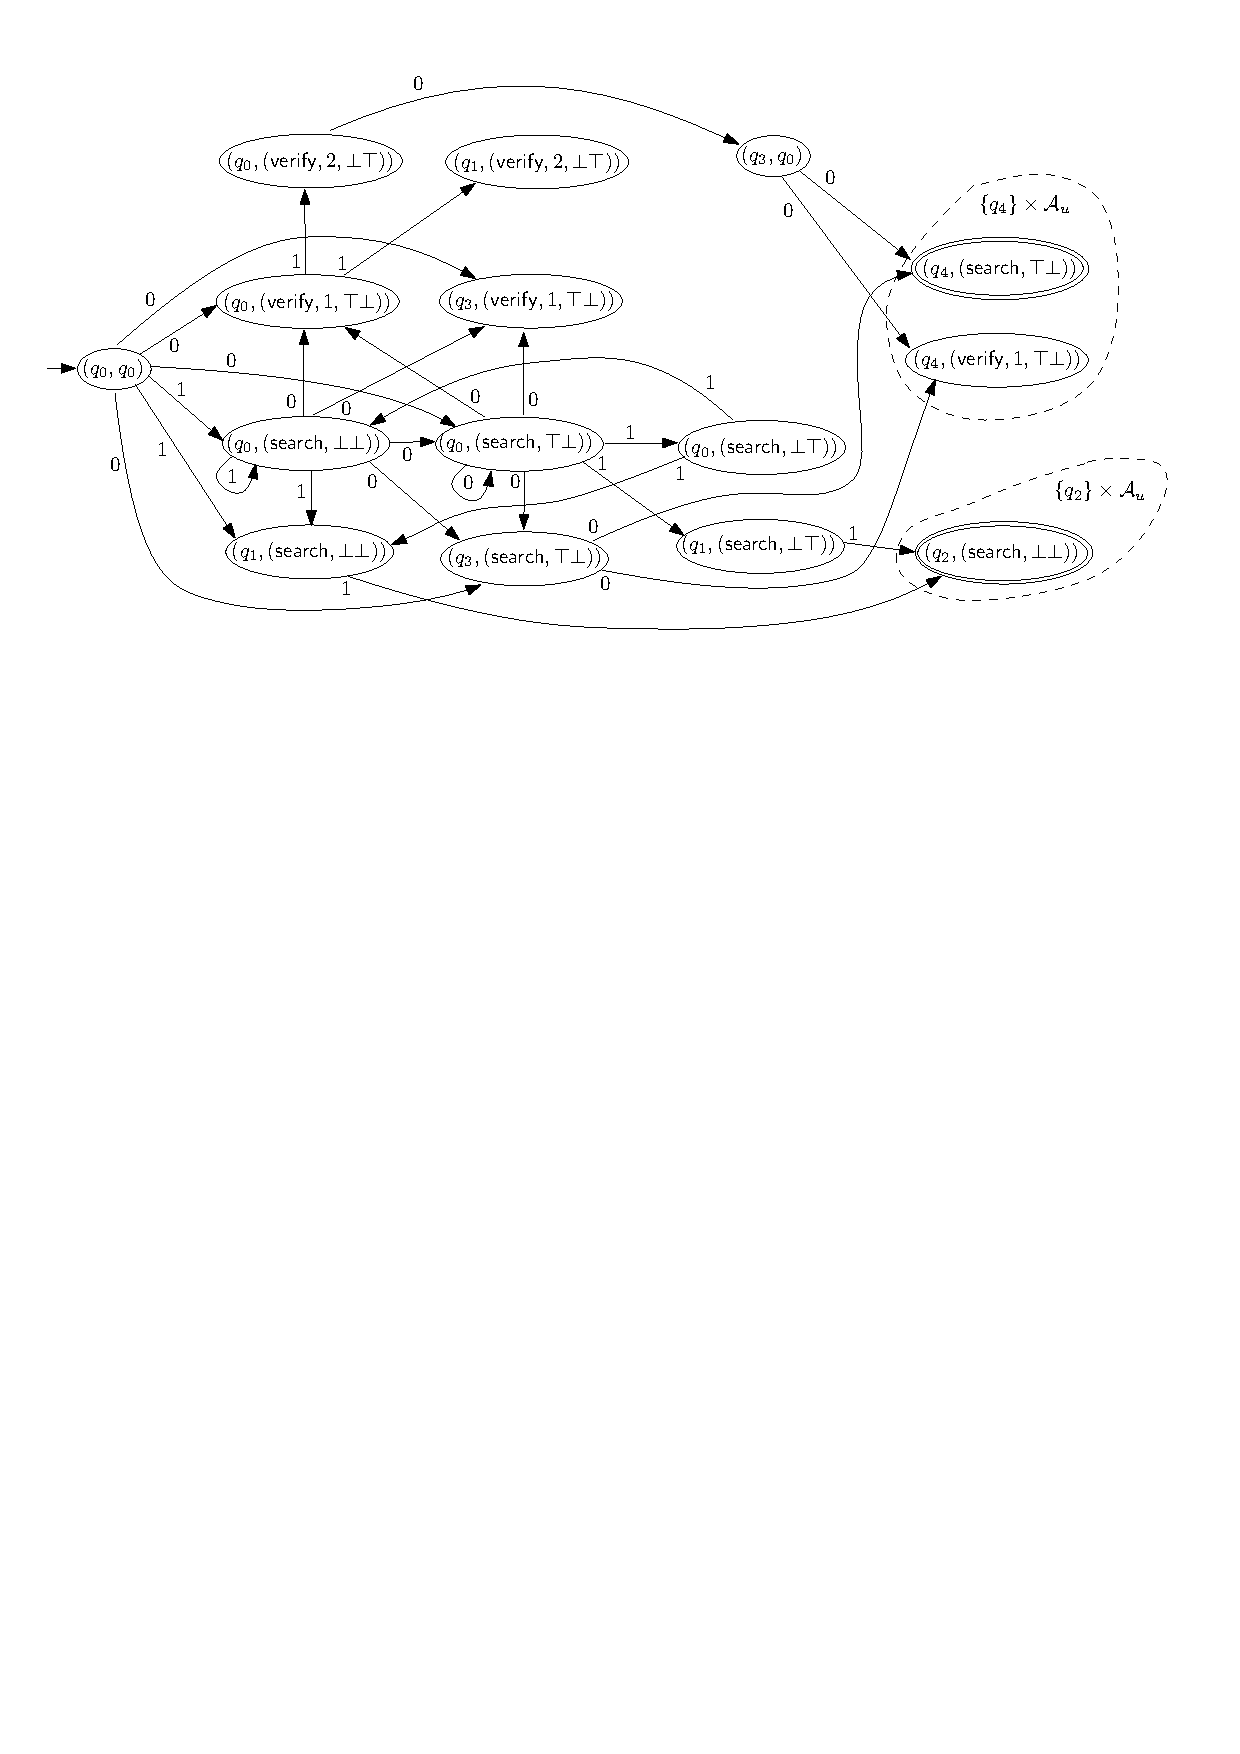
\includegraphics[scale=0.65]{constant-string-example.pdf}
\end{center}
\caption{The NFA $\cA_1 \times \cA_u$ for $u = 010$}\label{fig-cs-exmp}
\end{figure}
%

\def\refsecreplaceallcs{\ref{sec:replaceallcs}}
\section{Complexity analysis in Section~\protect\refsecreplaceallcs}
\label{sec:cs-complexity-full}

We provide a more detailed analysis of the complexity of the algorithm for the constant string case, described in Section~\ref{sec:replaceallcs}.
A summary of this argument already appears in Section~\ref{sec:replaceallcs}.

When constructing $G_{i+1}$ from $G_i$, suppose the two edges from $x$ to $y$ and $z$ respectively are currently removed, let the labels of the two edges be $({\sf l}, u)$ and $({\sf r}, u)$ respectively, then each element $(\cT, \cP)$ of $\cE_i(x)$ may be transformed into an element $(\cT', \cP')$ of $\cE_{i+1}(y)$ such that $|\cT'| = O(|u||\cT|)$, meanwhile, it may also be transformed into an element $(\cT'', \cP'')$ of $\cE_{i+1}(z)$ such that $\cT''$ has the same state space as $\cT$. Thus, for each source variable $x$, $\cE(x)$ contains at most exponentially many elements, and each of them may have a state space of at most exponential size. For instance, for a path from $x'$ to $x$ where the constant strings $u_1,\cdots, u_n$ occur in the labels of edges, an element $(\cT,\cP) \in \cE_0(x')$ may induce an element $(\cT', \cP')$ of $\cE(x)$ such that $|\cT'| \le |\cT| |u_1| \cdots |u_n|$, which is exponential in the worst case. 
%
To solve the nonemptiness problem of the intersection of all these regular constraints, the exponential space is sufficient. Consequently, in this case, we still obtain an EXPSPACE upper bound. 

Let us now consider the special situation that the $\rpleft$-length of $G_C$ is bounded by a constant $c$.
Since $\dmdidx(G_C) \le \lftlen(G_C)$, we know that $\dmdidx(G_C)$ is also bounded by $c$. Therefore, according to Proposition~\ref{prop-di}, there are at most polynomially different paths in $G_C$, we deduce that for each source variable $x$, $\cE(x)$ contains at most polynomially many elements. In addition, since the number of $\rpleft$-edges in each path is bounded by $c$, during the execution of the decision procedure, the number of times when $(\cT, \cP)$ of $\cE_i(x)$ may be transformed into an element $(\cT', \cP')$ of $\cE_{i+1}(y)$ such that $|\cT'| = O(|u||\cT|)$ is bounded by $c$.
Therefore, for each source variable $x$ and each element $(\cT'', \cP'')$ in $\cE(x)$,  $|\cT''|$ is at most polynomial in the size of $C$. We then conclude that for each source variable $x$, $\cE(x)$ corresponds to the intersection of polynomially many regular constraints such that each of them has a state space of polynomial size. Therefore, the nonemptiness of the intersection of all the regular constraints in $\cE(x)$ can be solved in polynomial space. In this situation, we obtain a PSPACE upper bound.


\def\refsecreplaceallre{\ref{sec:replaceallre}}
\section{Complexity analysis in Section~\protect\refsecreplaceallre}
\label{sec:re-complexity-full}

We provide a more detailed analysis of the complexity of the algorithm for the regular-expression case, described in Section~\ref{sec:replaceallre}.
A summary of this argument already appears in Section~\ref{sec:replaceallre}.

In each step of the reduction, suppose the two edges out of $x$ are currently removed, let the two edges be from $x$ to $y$ and $z$ and labeled by $({\sf l}, e)$ and $({\sf r}, e)$ respectively, then each element of $(\cT, \cP)$ of $\cE_i(x)$ may be transformed into an element $(\cT',\cP')$ of $\cE_{i+1}(y)$ such that $|\cT'| = |\cT| \cdot 2^{O(p(|e|))}$, meanwhile, it may also be transformed into an element $(\cT'',\cP'')$ of $\cE_{i+1}(y)$ such that $\cT''$ has the same state space as $\cT$. Thus, after the reduction, for each source variable $x$, $\cE(x)$ may contain exponentially many elements, and each of them may have a state space of exponential size, more precisely, if we start from a vertex $x$ without predecessors, with an element $(\cT,\cP)$ in $\cE_0(x)$, and go to a source variable $y$ through a path where $k$ edges have been traversed and removed, let $e_1,\cdots, e_k$ be the regular expressions occurring in the labels of these edges, then the resulting element in $\cE(y)$ has a state space of size $|\cT| \cdot 2^{O(p(|e_1|))} \cdot 2^{O(p(|e_2|))} \cdot \cdots \cdot 2^{O(p(|e_k|))}$ in the worst case. To solve the nonemptiness problem of the intersection of all these regular constraints, the exponential space is sufficient. Consequently, for the most general case of regular expressions, we still obtain a EXPSPACE upper bound. 

On the other hand, for the situation that the $\rpleft$-length of $G_C$ is at most one, we wan to show that the algorithm runs in polynomial space. Suppose the $\rpleft$-length of $G_C$ is at most one. Then the diamond index of $G_C$ is at most one as well. According to Proposition~\ref{prop-di}, there are only polynomially many paths in $G_C$. Nevertheless, for each source variable $x$, $\cE(x)$ may contain an element $(\cT,\cP)$ such that $|\cT|$ is exponential. Since $|\cP|$ may be exponential, $(\cT,\cP)$ may correspond to the intersection of exponentially many regular constraints. However, we can show that $|\cP|$ is at most polynomial, as a result of the fact that the $\rpleft$-length of $G_C$ is at most one. The arguments proceed as follows: Suppose two edges from $x$ to $y, z$ respectively are removed, and an element $(\cT', \cP')$ of $\cE_{i+1}(y)$ such that $|\cT'|$ is exponential and $|\cP'|$ is polynomial, is generated from an element of $(\cT, \cP)$ of $\cE_i(x)$. Then $y$ must be a source variable in $G_C$. Otherwise, there is an $\rpleft$-edge out of $y$ and the $\rpleft$-length of $G_C$ is at least two, a contradiction. Therefore, $y$ is a source variable in $G_C$, $(\cT', \cP')$  will not be used to generate the regular constraints for the other variables. In other words, $y$ is a source variable in $G_C$, and $(\cT', \cP') \in \cE(y)$ with $|\cP'|$ polynomial. We then conclude that for each source variable $x$, $|\cE(x)|$  is at most polynomial in the size of $C$ and for each element $(\cT, \cP) \in \cE(x)$, $|\cP|$ is polynomial in the size of $C$. Therefore, for each source variable $x$,  $\cE(x)$ corresponds to the intersection of polynomially many regular constraints, where each of them has a state space at most exponential size. To solve the nonemptiness of the intersection of these regular constraints, the polynomial space is sufficient. We obtain a PSPACE upper bound for the situation that the $\rpleft$-length of $G_C$ is at most one.


\def\refsecext{\ref{sec-ext}}
\section{Undecidability Proofs for Section~\protect\refsecext}
\label{sec:ext-undec-proofs}

\subsection{Proof of Theorem~\ref{thm-ext-int}}

\begin{proof}
	The basic idea of the reduction is to simulate the two polynomials $f(x_1,\cdots, x_n)$ and $g(x_1,\cdots, x_n)$, where $x_1,\cdots,x_n$ range over the set of natural numbers, with two $\strline[\concat,\replaceall]$ formulae $C_f, C_g$ over a unary alphabet $\{a\}$, with the output string variables $y_f, y_g$ respectively, and simulate the equality $f(x_1,\cdots, x_n) = g(x_1,\cdots, x_n)$ with the integer constraint $|y_f|=|y_g|$ (which is equivalent to $y_f = y_g$, since $y_f, y_g$ represent strings over the unary alphabet $\{a\}$). 
	
	A polynomial $f(x_1,\cdots, x_n)$ or $g(x_1,\cdots, x_n)$ where $x_1, \cdots, x_n$ range over the set of natural numbers, can be simulated by an $\strline[\concat,\replaceall]$ formula over an unary alphabet $\{a\}$ as follows: The natural numbers are represented by the strings over the alphabet $\{a\}$. A string variable is introduced for each subexpression of $f(x_1,\cdots, x_n)$. The numerical addition operator $+$ is simulated by the string operation $\concat$ 
	%\mat{$\concat$ is not part of $\strline[\replaceall]$, can it be simulated when the string alphabet is unary, or do we need two extra characters?}\zhilin{changed to $\strline[\concat,\replaceall]$.}
	and the multiplication operator $*$ is simulated by $\replaceall$. Since it is easy to figure out how the simulation proceeds, we will only use an example to illustrate it and omit the details here. Let us consider $f(x_1,x_2) = x_1^2 + 2 x_1 x_2 + 5$. By abusing the notation, we also use $x_1,x_2$ as string variables in the simulation. We will introduce a string variable for each subexpression in $f(x_1,x_2)$, namely the variables $y_{x_1^2}, y_{x_1x_2}, y_{2x_1x_2}, y_{x_1^2+2x_1x_2}, y_{f(x_1,x_2)}$. Then $f(x_1,x_2)$ is simulated by the $\strline[\concat,\replaceall]$ formula
	\[
	\begin{array} {l c l }
	C_f & \equiv & y_{x_1^2} = \replaceall(x_1,a, x_1)\ \wedge y_{x_1x_2} = \replaceall(x_1, a, x_2)\ \wedge \\
	& & y_{2x_1x_2} = \replaceall(aa, a, y_{x_1x_2})\ \wedge y_{x_1^2+2x_1x_2} = y_{x_1^2} \concat y_{2x_1x_2}\ \wedge  \\
	& & y_{f(x_1,x_2)}=y_{x_1^2+2x_1x_2} \concat a a a a a\ \wedge x_1 \in a^*\ \wedge x_2 \in a^*.
	\end{array}
	\]
	Then according to Proposition~\ref{prop-concat}, $C_f, C_g$ can be turned into equivalent $\strline[\replaceall]$ formula $C'_f, C'_g$ by introducing fresh letters.
	%\mat{But we may have to give up the unary alphabet?}\zhilin{yes, you are  right, it is fine.}
	
	Since $C'_f$ and $C'_g$ share only source variables $x_1,\cdots, x_n$, we know that $C'_f \wedge C'_g$ is still an $\strline[\replaceall]$ formula.
	From the construction of $C'_f, C'_g$, it is evident that for every pair of polynomials $f(x_1,\cdots, x_n)$ and $g(x_1,\cdots, x_n)$, $f(x_1,\cdots, x_n) = g(x_1,\cdots, x_n)$ has a solution in natural numbers iff $C'_f \wedge C'_g \wedge |y_f| = |y_g|$ is satisfiable. The proof is complete.
	%
	%%%%%%%%%%%%%%%%%%%%%%%%%%%%%%%%%%%%%%%%%%%%%%%%%%%%%%%%%%%
	%%%%%%%%%%%%%%%%%%%%%%%%%%%%%%%%%%%%%%%%%%%%%%%%%%%%%%%%%%%
	\hide{
		We shall reduce from the aforementioned version of the Hilbert tenth problem. For any polynomial with positive integral  $f(x_1, \cdots, x_n)$ where each coefficient is a positive, we can construct a (division-free) arithmetic circuit (AC) is a directed  acyclic graph with nodes labelled with constants from $\mathbb{Z}$, or with some indeterminates $X_1, \cdots, X_m$, or with the operators $+, -, *$. The nodes labelled with constants are called constant nodes, while those labelled with indeterminates are called input nodes. Both constant and input nodes do not have incoming edges. Internal nodes are those labelled with $+,-,*$. Output node is the one which does not have out-going edges. Without loss of generality we assume that each internal node has in-degree 2, and there is only one output node. Each node in the circuit represents a multivariate polynomial $\mathbb{Z}[X_1, \cdots, X_m]$. Vice verse, each polynomial $f\in \mathbb{Z}[X_1, \cdots, X_m]$ can be represented as an AC, and, if the polynomial has only positive (integral) coefficients, the corresponding AC does not contain nodes labelled by $-$ or negative constants.  
		
		We observe that, given an AC, one can construct an SL[$\concat, \replaceall$] formula over the alphabet $\Sigma=\{a\}$ as follows. Each node $n$ of the AC is associated with a string variable $x_n$. As a result, each input node of the AC labelled by $X_i$ (i.e., the indeterminate) corresponds to a  source variable.   
		\begin{itemize}
			\item For each internal node $n$ labelled by $+$, suppose that $n$ has two children nodes $n_l$ and $n_r$, we introduce a string constraint $x_n= x_{n_l}\concat x_{n_l}$.  
			
			\item For each internal node $n$ labelled by $*$, suppose that $n$ has two children nodes $n_l$ and $n_r$, we introduce a string constraint $x_n= \replaceall(x_{n_l}, a, x_{n_l})$.  		
		\end{itemize}
		Furthermore, we introduce, for each node $n$ labelled by a constant $c$, a regular constraint $x_n=a^c$. 
		
		It is straightforward to verify, according to the semantics of SL[$\concat, \replaceall$], that:
		\begin{itemize}
			\item for relational constraint $x_n= x_{n_l}\concat x_{n_l}$, $|x_n|= |x_{n_l}|+|x_{n_l}|$; 
			\item for relational constraint $x_n= \replaceall(x_{n_l}, a, x_{n_l})$,  $|x_n|= |x_{n_l}|\cdot |x_{n_l}|$; and 
			\item for regular $x_n=a^c$, $|x_n|=c$. 
		\end{itemize}
		
		It follows that for each polynomial $f(x_1, \cdots, x_m)$ with positive integral coefficients, we can construct a straight-line string constraint $\varphi_{f}\wedge\psi_g$ over $\Sigma=\{a\}$ with $y_f$ as the output variant and $y_1, \cdots, y_n$ as source variables such that
		$f(c_1, \cdots, c_m)=|y|$ and, for each $1\leq i\leq m$, $|y_i|= c_i$ (i.e., $y_i=a^{c_i}$).  
		
		Consequently, when given two polynomials $f(x_1, \cdots, x_m)$ and $g(x_1, \cdots, x_m)$, we have straight-line string constraints $\varphi_{f}\wedge \varphi_{g}\wedge \psi_{f}\wedge \psi_g$ with two distinguished two variables  $y_f$ and $y_g$ such that  
		\[\exists x_1, \cdots, x_m. f(x_1, \cdots, x_m)=g(x_1, \cdots, x_m)\mbox{ iff } |y_f|=|y_g|\wedge \varphi_{f}\wedge \varphi_{g}\wedge \psi_{f}\wedge \psi_g\mbox{ is satisfiable} \]
		
		Finally, note that any  SL[$\concat, \replaceall$] constraints can be transformed into SL[$\replaceall$] constraints, we obtain a reduction from the Hilbert's 10th problem to the satisfiability problem of  SL[$\replaceall$] with length constraints, which entail that the latter problem is undecidable. The proof is completed. 
	}
	%%%%%%%%%%%%%%%%%%%%%%%%%%%%%%%%%%%%%%%%%%%%%%%%%%%%%%%%%%%
	%%%%%%%%%%%%%%%%%%%%%%%%%%%%%%%%%%%%%%%%%%%%%%%%%%%%%%%%%%%
\end{proof}

\subsection{Undecidability of Depth-1 dependency graph}

A \emph{linear polynomial} (resp.\ quadratic polynomial) is a polynomial with degree at most one (resp.\ with degree at most two) where each coefficient is an integer. %of the form $a_0 + a_1x_1 + \cdots + a_n x_n$ (resp. a polynomial with degree at most two) where each coefficient $a_i\in \mathbb{Z}$  for $0 \leq i \leq n$. A quadratic polynomial

\begin{theorem}[\cite{ID04}]\label{thm-quad-eq}
	%	There exists some (fixed) $k$ such that no algorithm can solve Diophantine systems in the following form
	%	\[y_1F_1=G_1, t_1H_1=I_1, \cdots, t_kF_k = G_k, t_kH_k = I_k,\] 
	%
	%	where $F_i, G_i, H_i, I_i$ for $1\leq i\leq k$ are nonnegative linear polynomials over natural number variables  $s_1, \cdots, s_m$.
	The following problem is undecidable: Determine whether a system of equations of the following form has a solution in natural numbers, 
	\[
	\begin{array} {l l }
	A_i = B_i, & i =1, \cdots, k,\\
	y_iF_i=G_i \wedge y_i H_i = I_i, & i =1, \cdots, m, 
	\end{array}
	\] 
	%
	where $A_i, B_i, F_i, G_i$ are linear polynomials on the variables $x_1,\cdots, x_n$ (Note that each variable $y_i$ occurs in exactly two quadratic equations).
\end{theorem}

We can get a reduction from the problem in Theorem~\ref{thm-quad-eq} to the satisfiability of the extension of $\strline[\replaceall]$ with integer constraints as follows: For each monomial $y_i x_j$ in the quadratic polynomials, we use an $\strline[\replaceall]$ formula $z_{y_i x_j} = \replaceall(y_i, a, x_j)$ to simulate $y_i x_j$, where $z_{y_i x_j}$ are freshly introduced string variables. Since each equation $y_iF_i=G_i$ or $y_i H_i = I_i$ can be seen as a linear combination of the terms $y_i x_j$ and $x_j$ for $i \in [m]$ and $j \in [n]$, we can replace each variable $x_j$ with $|x_j|$, and each term $y_ix_j$ with $|z_{y_i x_j}|$,  thus transform them into the (linear) integer constraints $F'_i = G'_i$ or $H'_i = I'_i$. Similarly, after replacing each variable $x_j$ with $|x_j|$, we transform each equation $A_i= B_i$ into an integer constraint $A'_i = B'_i$. Therefore, we get a formula 
$$
\begin{array}{l c l }
\bigwedge \limits_{i \in [m], j \in [n]} z_{y_i x_j} = \replaceall(y_i, a, x_j) \wedge \bigwedge \limits_{i \in [m]} y_i \in a^*\ \wedge  \bigwedge \limits_{j \in [n]} x_j \in a^* \  \wedge\\
\hspace{2cm} \bigwedge \limits_{i \in [k]} A'_i = B'_i \wedge \bigwedge \limits_{i \in [m]} (F'_i = G'_i \wedge H'_i = I'_i),
\end{array}
$$
where the dependency graph of the $\strline[\replaceall]$ subformula is of depth at most one.

%%%%%%%%%%%%%%%%%%%%%%%%%%%%%%%%%%%%%%%%%%%%%%%%%
%%%%%%%%%%%%%%%%%%%%%%%%%%%%%%%%%%%%%%%%%%%%%%%%%
\hide{
	From this class of quadratic Diophantine equations, we can introduce string variables $x_1, \cdots, x_k$ and $y_1, \cdots, y_m$, together with relational string constraints 
	\[z_{i,j}=\replaceall(x_i, a, y_j)\]
	for $1\leq i\leq k$ and $1\leq j\leq m$. Note that, for each $i$,  $t_i F_i=G_i$ can be written as
	\begin{equation} \label{eq:dio}
	t_i\cdot \left(a_0+\sum_{j=1}^s a_j s_j\right) =  b_0+\sum_{j=1}^s b_j s_j
	\end{equation}
	where $a$'s and $b$'s are all natural numbers. Moreover, \eqref{eq:dio} holds iff 
	\[a_0\cdot |y_i|+ \sum_{j=1}^s a_j |z_{i,j}| =  b_0+ \sum_{j=1}^s b_j |x_j| \] 
	which is an integer constraint defined in Definition~\ref{def:intconst}. This entails that
}
%%%%%%%%%%%%%%%%%%%%%%%%%%%%%%%%%%%%%%%%%%%%%%%%%
%%%%%%%%%%%%%%%%%%%%%%%%%%%%%%%%%%%%%%%%%%%%%%%%%

\subsection{Undecidability of the character constraints}

\begin{proposition}\label{prop-ext-char}
	For the extension of $\strline[\replaceall]$ with character constraints, the satisfiability problem is undecidable. 
\end{proposition}

The arguments for Proposition~\ref{prop-ext-char} proceed as follows. Recall that in the proof of Theorem~\ref{thm-ext-int}, we get a formula $C_f \wedge C_g \wedge |y_f| = |y_g|$ such that $f(x_1,\cdots, x_n) = g(x_1,\cdots, x_n)$ has a solution in natural numbers iff $C_f \wedge C_g \wedge |y_f| = |y_g|$ is satisfiable. Let $\$ \neq a$. Suppose  $z_f = y_f \concat \$$, and $z_g = y_g \concat \$$. Then $|y_f| = |y_g|$ can be captured by $z_f[\mathfrak{n}] = \$[1] \wedge  z_g[\mathfrak{n}] = \$[1]$, where $\mathfrak{n}$ is a variable of type $\intnum$. More precisely, 
%
we have 
\begin{quote}
	\centering
	$C_f \wedge C_g \wedge |y_f|= |y_g|$ is satisfiable \\
	%
	iff \\
	%
	$C_f \wedge C_g \wedge z_f = y_f \concat \$ \wedge z_g = y_g \concat \$ \wedge z_f[\mathfrak{n}] = \$[1] \wedge  z_g[\mathfrak{n}] = \$[1]$ is satisfiable. 
\end{quote}
Therefore, we get a reduction from Hilbert's tenth problem to the satisfiability problem for the extension of $\strline[\replaceall]$ with character constraints. 

%For any two string variables $x,y$ on the unary alphabet $\{a\}$, let $x' = x \concat \$$ and $y' = y \concat \$$, then $|x| = |y|$ iff .
%
% $|x|=|y|$ iff $\exists n. x[n]=y[n]=\$$. 
%
%
%\begin{lemma}
%	For any two strings $x,y\in a^*\$$, $|x|=|y|$ iff $\exists n. x[n]=y[n]=\$$. 
%\end{lemma}
%
%As SL[$\replaceall$] with length constraints is undecidable, we conclude that 
%
%
%
%\tl{I am not satisfied with this as the quantifier is used}

\subsection{Undecidability of the $\indexof$ constraints}

\begin{proposition}\label{prop-indexof}
	For the extension of $\strline[\replaceall]$ with the $\indexof$ constraints, the satisfiability problem is undecidable. 
\end{proposition}

Proposition~\ref{prop-ext-char} follows from the following observation and Theorem~\ref{thm-ext-int}: For any two string variables $x,y$ over a unary alphabet, 
$1= \indexof(x,y)$ iff $x$ is a prefix of $y$. Therefore, $|x| = |y|$ iff $1=  \indexof(x,y) \wedge 1= \indexof(y,x)$. This implies that in the proof of Theorem~\ref{thm-ext-int}, we can replace $|y_f| = |y_g|$ with $1=\indexof(y_f, y_g) \wedge 1 = \indexof(y_g, y_f)$ and get a reduction from Hilbert's tenth problem to the satisfiability problem for the extension of $\strline[\replaceall]$ with the $\indexof$ constraints.
Note that $=$ can be simulated as a conjunction of $\leq$ and $\geq$.


%We have the following observation: 
%\begin{lemma}
%	For any two strings $x,y$ over $\{a\}$, $x=y$ iff $1=\indexof(x,y)=\indexof(y,x)$.  
%\end{lemma}
%
%It follows that 

%\subsection*{Further undecidability results}


\def\refsecreplaceallre{\ref{sec:replaceallre}}
\section{Examples in Section~\protect\refsecreplaceallre}

\begin{example}\label{exmp-pa-re}
	Let $e_0 = 0^*0 1(1^* + 0^*)$. Then $\cA_{0}$ and $\cA_{e_0}$ are illustrated in Figure~\ref{fig-pa-re}, where ${\sf sleft}$ and ${\sf slong}$ are the abbreviations of $\searchleft$ and $\searchlong$ respectively. Let us use the state $(\{q_{0,1}\}\{q_{0,0}\}, {\sf sleft}, \emptyset)$ to illustrate the construction. Since $\big(\delta_0(\{q_{0,1}\}, 0) \cup \delta_0(\{q_{0,0}\}, 0)\big) \cap F_0 = \{q_{0,1}\} \cap F_0 = \emptyset$, $\delta_0(\emptyset, 0) \cap F_0 = \emptyset$, and $\red(\delta_0(\{q_{0,1}\}, 0) \delta_0(\{q_{0,0}\}, 0))=\{q_{0,1}\}$, we deduce that the transition $((\{q_{0,1}\}\{q_{0,0}\}, {\sf sleft}, \emptyset), 0, (\{q_{0,1}\} \{q_{0,0}\}, {\sf sleft}, \emptyset)) \in \delta_{e_0}$. On the other hand, it is impossible to go from the state $(\{q_{0,1}\}\{q_{0,0}\}, {\sf sleft}, \emptyset)$ to the ``$\searchlong$'' mode. This is due to the fact that $\delta_0(\{q_{0,0}\}, 0)=\{q_{0,1}\} \subseteq \delta_0(\{q_{0,1}\},0)=\{q_{0,1}\}$. In addition, there are no $1$-transitions out of $(\{q_{0,1}\}\{q_{0,0}\}, {\sf sleft}, \emptyset)$. This is due to the fact that $\delta_0(\{q_{0,1}\}, 1) \cap F_0 = \{q_{0,2}, q_{0,3}\} \cap F_0 \neq \emptyset$.
	%
	\begin{figure}[htbp]
		\begin{center}
			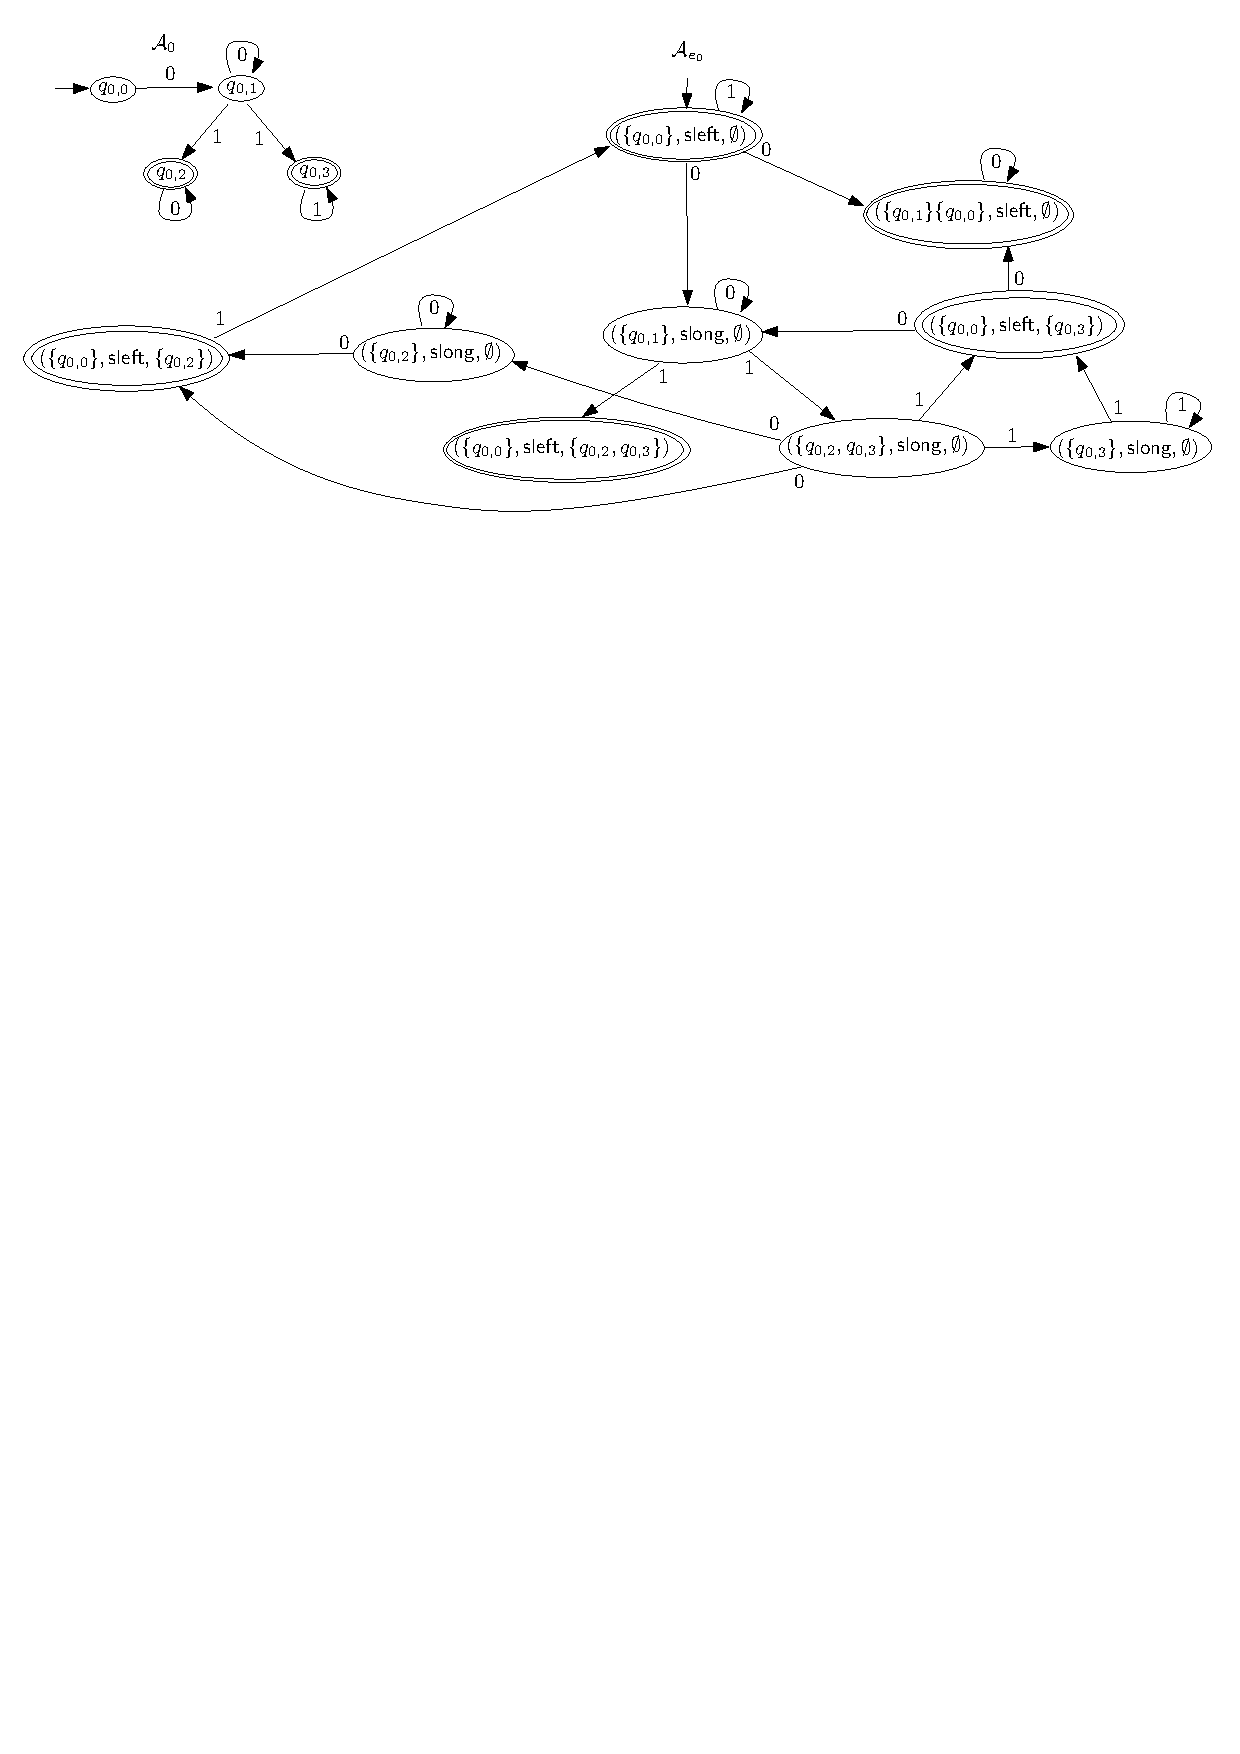
\includegraphics[scale=0.7]{regular-expression-example.pdf}
		\end{center}
		\caption{The NFA $\cA_0$ and $\cA_{e_0}$ for $e_0 = 0^*0 1(1^* + 0^*)$}\label{fig-pa-re}
	\end{figure} 
\end{example}

\begin{example}
	Let $C \equiv x = \replaceall(y, e_0, z) \wedge x \in e_1 \wedge y \in e_2 \wedge z \in e_3$, where $e_1,e_2,e_3$ are as in Example~\ref{exmp-sl} (cf. Figure~\ref{fig-sl-exmp}) and $e_0$ is as in Example~\ref{exmp-pa-re} (cf. Figure~\ref{fig-pa-re}). Suppose $T_z = \{(q_0, q_0), (q_1, q_2)\}$. Then the NFA $\cB_{\cA_1, e_0, T_z}$ is as illustrated in Figure~\ref{fig-re-exmp}, where the thick edges denote the added transitions. Let us use the state $(q_1, (\{q_{0,0}\}, \searchleft, \emptyset))$ to exemplify the construction. The transition $((q_1, (\{q_{0,0}\}, \searchleft, \emptyset)), 1, (q_2, (\{q_{0,0}\}, \searchleft, \emptyset)))$ is  in $\cA_1 \times \cA_{e_0}$. Since $\delta_0(q_{0,0}, 1) \cap F_0 = \emptyset$, this transition is not removed and is thus in $\cB_{\cA_1, e_0, T_z}$. On the other hand, since there are no $0$-transitions out of $q_1$ in $\cA_1$, there are no $0$-transitions from $(q_1, (\{q_{0,0}\}, \searchleft, \emptyset))$ to some state from $Q_{\searchleft}$ in $\cB_{\cA_1, e_0, T_z}$. 
	Moreover, because $((\{q_{0,0}\}, \searchleft, \emptyset), 0, (\{q_{0,1}\}, \searchlong, \emptyset)) \in \delta_{e_0}$ and $(q_1, q_2) \in T_z$, the transition $((q_1, (\{q_{0,0}\}, \searchleft, \emptyset)), 0, (q_1, (\{q_{0,1}\}, \searchlong, \emptyset)))$ is added. 
	One may also note that there are no 0-transitions from $(q_2, (\{q_{0,0}\}, \searchleft, \emptyset))$ to the state $(q_2, (\{q_{0,1}\}, \searchlong, \emptyset))$, because there are no pairs $(q2,-) \in T_z$.
	It is not hard to see that $010101 \in \Ll(\cA_2) \cap \Ll(\cB_{\cA_1, e_0, T_z})$. In addition, $10 \in \Ll(\cA_3) \cap \Ll(\cA_1(q_0,q_0)) \cap \Ll(\cA_1(q_1,q_2))$. Let $y$ be $010101$ and $z$ be $10$. Then $x$ takes the value $\replaceall(010101, e_0, 10)=10 \cdot \replaceall(101, e_0, 10)=10110$, which is accepted by $\cA_1$. Therefore, $C$ is satisfiable.
	\begin{figure}[htbp]
		\begin{center}
			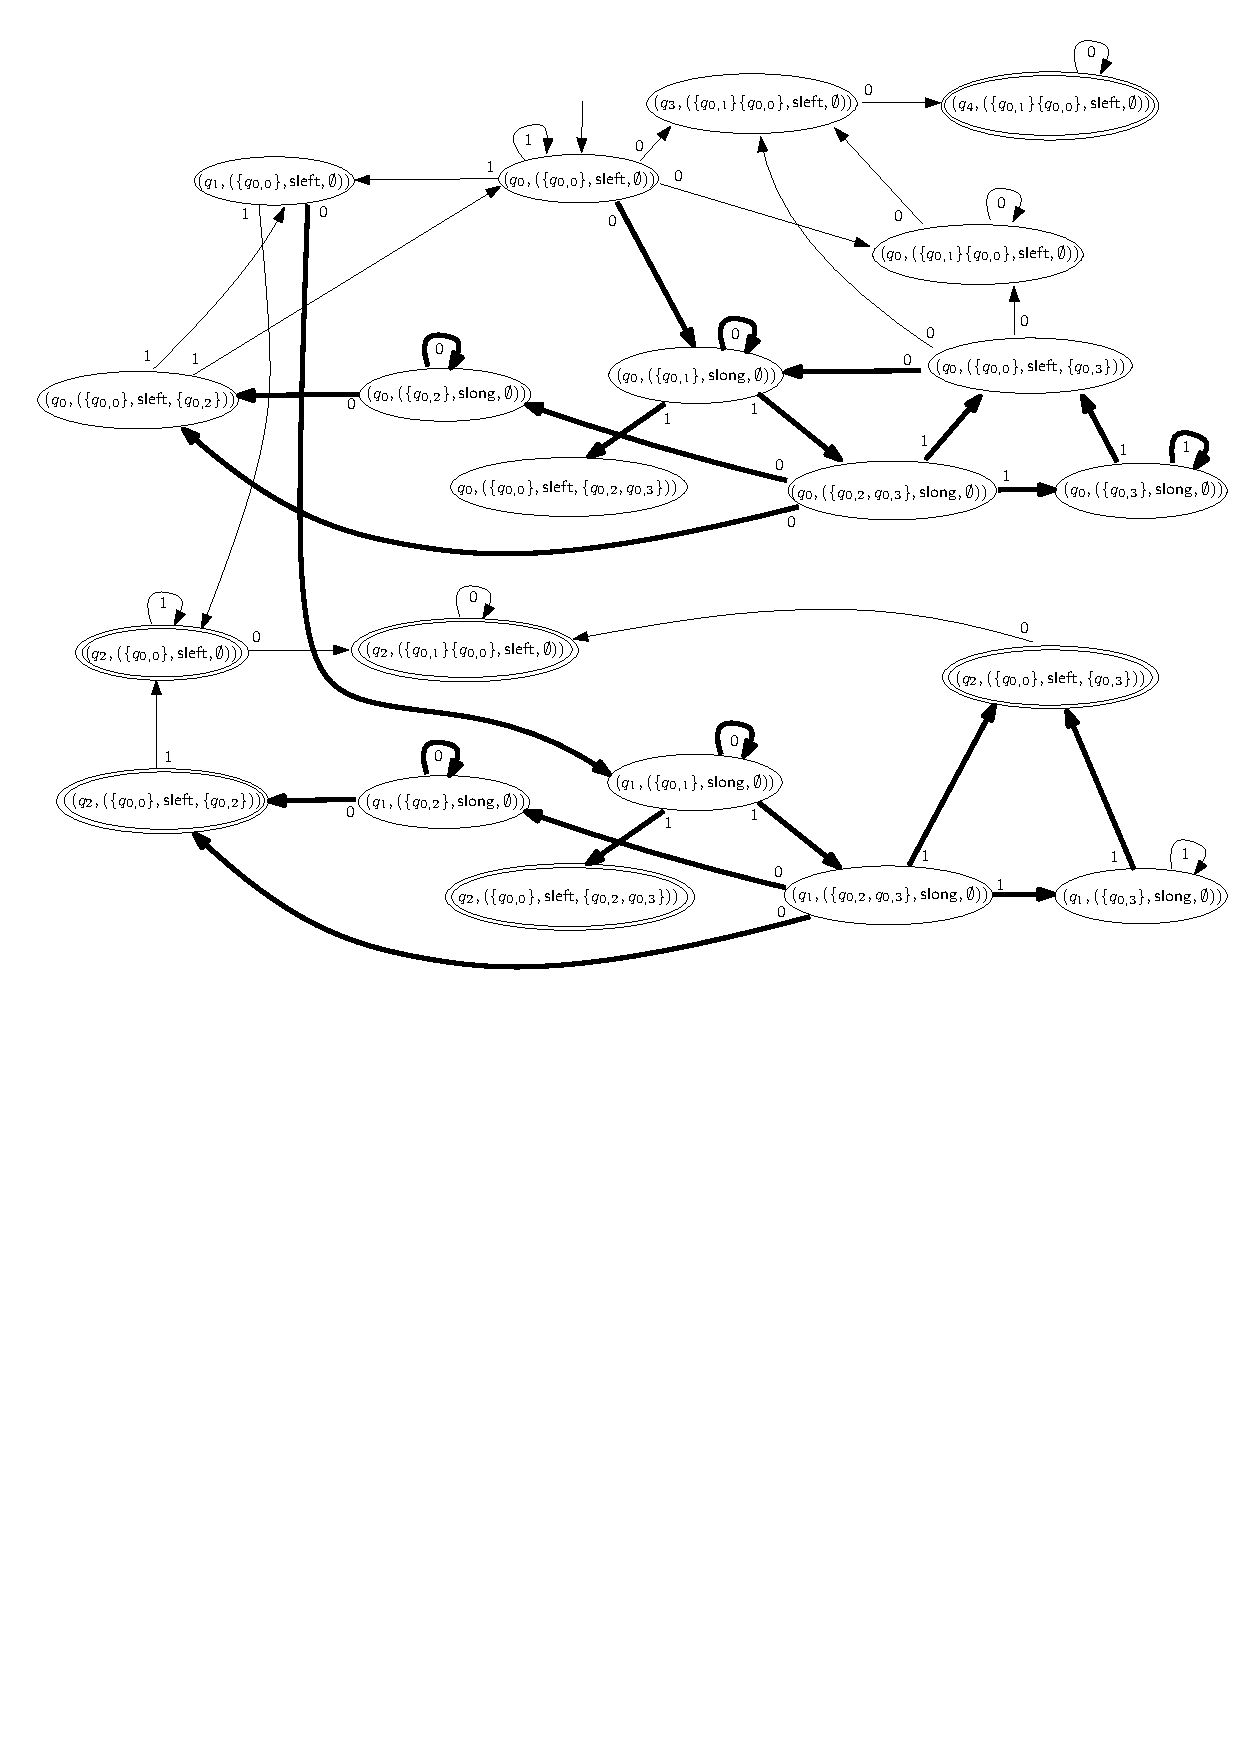
\includegraphics[scale=0.68]{regular-expression-example-2.pdf}
		\end{center}
		\caption{The NFA $\cB_{\cA_1, e_0, T_z}$}\label{fig-re-exmp}
	\end{figure} 
\end{example}


\end{appendix}

\fi

\end{document}
